\documentclass[11pt]{article}
%DIF LATEXDIFF DIFFERENCE FILE
%DIF DEL /tmp/claude-1000/-home-bijanf-Documents-AMOC-renalysis-PAPER-3-v2/9cb18994-7a7e-41de-afa6-ede6a2d815b2/scratchpad/baseline/Main.tex   Wed Aug  5 13:34:03 2026
%DIF ADD /home/bijanf/Documents/AMOC_renalysis/PAPER_3_v2/Main.tex                                                                             Wed Aug  5 12:51:37 2026

\usepackage[margin=2.4cm]{geometry}
\usepackage[T1]{fontenc}
\usepackage[utf8]{inputenc}
\usepackage{lmodern}
\usepackage{amsmath}
\usepackage{graphicx}
\usepackage{booktabs}
\usepackage{caption}
\usepackage[numbers,super,sort&compress]{natbib}
\usepackage{lineno}
\usepackage[colorlinks=true,allcolors=black]{hyperref}

\graphicspath{{figures/}}

\captionsetup{
  font=small,
  labelfont=bf,
  labelsep=period,
  justification=justified,
  singlelinecheck=false
}

\setlength{\parindent}{0pt}
\setlength{\parskip}{0.6em}
\linespread{1.15}

\newcommand{\Fovs}{F_{\mathrm{ov}}^{S}}
\newcommand{\degree}{$^\circ$}
\newcommand{\degS}{$^\circ$S}
\newcommand{\degN}{$^\circ$N}
\newcommand{\degW}{$^\circ$W}
\newcommand{\degE}{$^\circ$E}

\title{\vspace{-2.0cm}\bfseries \DIFdelbegin \DIFdel{Negative Atlantic freshwater }\DIFdelend \DIFaddbegin \DIFadd{The declining Atlantic overturning freshwater
transport at 34.5$^\circ$S is not explained by a declining overturning
}\DIFaddend transport\DIFdelbegin \DIFdel{is robust
across ocean reanalyses, but its decline does not track the overturning
}\DIFdelend }

\author{}
\date{}
%DIF PREAMBLE EXTENSION ADDED BY LATEXDIFF
%DIF UNDERLINE PREAMBLE %DIF PREAMBLE
\RequirePackage[normalem]{ulem} %DIF PREAMBLE
\RequirePackage{color}\definecolor{RED}{rgb}{1,0,0}\definecolor{BLUE}{rgb}{0,0,1} %DIF PREAMBLE
\providecommand{\DIFaddtex}[1]{{\protect\color{blue}\uwave{#1}}} %DIF PREAMBLE
\providecommand{\DIFdeltex}[1]{{\protect\color{red}\sout{#1}}}                      %DIF PREAMBLE
%DIF SAFE PREAMBLE %DIF PREAMBLE
\providecommand{\DIFaddbegin}{} %DIF PREAMBLE
\providecommand{\DIFaddend}{} %DIF PREAMBLE
\providecommand{\DIFdelbegin}{} %DIF PREAMBLE
\providecommand{\DIFdelend}{} %DIF PREAMBLE
\providecommand{\DIFmodbegin}{} %DIF PREAMBLE
\providecommand{\DIFmodend}{} %DIF PREAMBLE
%DIF FLOATSAFE PREAMBLE %DIF PREAMBLE
\providecommand{\DIFaddFL}[1]{\DIFadd{#1}} %DIF PREAMBLE
\providecommand{\DIFdelFL}[1]{\DIFdel{#1}} %DIF PREAMBLE
\providecommand{\DIFaddbeginFL}{} %DIF PREAMBLE
\providecommand{\DIFaddendFL}{} %DIF PREAMBLE
\providecommand{\DIFdelbeginFL}{} %DIF PREAMBLE
\providecommand{\DIFdelendFL}{} %DIF PREAMBLE
%DIF HYPERREF PREAMBLE %DIF PREAMBLE
\providecommand{\DIFadd}[1]{\texorpdfstring{\DIFaddtex{#1}}{#1}} %DIF PREAMBLE
\providecommand{\DIFdel}[1]{\texorpdfstring{\DIFdeltex{#1}}{}} %DIF PREAMBLE
%DIF COLORLISTINGS PREAMBLE %DIF PREAMBLE
\RequirePackage{listings} %DIF PREAMBLE
\RequirePackage{color} %DIF PREAMBLE
\lstdefinelanguage{DIFcode}{ %DIF PREAMBLE
%DIF DIFCODE_UNDERLINE %DIF PREAMBLE
  moredelim=[il][\color{red}\sout]{\%DIF\ <\ }, %DIF PREAMBLE
  moredelim=[il][\color{blue}\uwave]{\%DIF\ >\ } %DIF PREAMBLE
} %DIF PREAMBLE
\lstdefinestyle{DIFverbatimstyle}{ %DIF PREAMBLE
	language=DIFcode, %DIF PREAMBLE
	basicstyle=\ttfamily, %DIF PREAMBLE
	columns=fullflexible, %DIF PREAMBLE
	keepspaces=true %DIF PREAMBLE
} %DIF PREAMBLE
\lstnewenvironment{DIFverbatim}{\lstset{style=DIFverbatimstyle}}{} %DIF PREAMBLE
\lstnewenvironment{DIFverbatim*}{\lstset{style=DIFverbatimstyle,showspaces=true}}{} %DIF PREAMBLE
%DIF END PREAMBLE EXTENSION ADDED BY LATEXDIFF

\begin{document}

\maketitle
\thispagestyle{empty}
\vspace{-2.2cm}

\linenumbers

\section*{Abstract}

Freshwater transport by the overturning at the southern boundary of the
Atlantic, $\Fovs$, is the standard \DIFdelbegin \DIFdel{diagnostic for }\DIFdelend \DIFaddbegin \DIFadd{indicator of }\DIFaddend whether the salt-advection
feedback is self-reinforcing, and its recent decline in ocean reanalyses \DIFdelbegin \DIFdel{has
been read as evidence of a weakening overturning . We evaluate }\DIFdelend \DIFaddbegin \DIFadd{is
increasingly read as a warning that the overturning is weakening. We show that
it is not. Once the net throughflow is removed, }\DIFaddend $\Fovs$ \DIFdelbegin \DIFdel{at
}\DIFdelend \DIFaddbegin \DIFadd{factorises exactly as
$-T\,\Delta S/S_0$, with $T$ the northward-limb volume transport and $\Delta S$
the transport-weighted salinity difference between the limbs, both measured
directly from the section. At }\DIFaddend 34.5\DIFdelbegin \DIFdel{\degS{} in four reanalyses spanning three ocean models and four
assimilation schemes. All four give a negative record mean, three with
block-bootstrap intervals that exclude zero, placing the modern Atlantic on the side of the freshwater budget where multiple equilibria are theoretically
possible. The decline is a different quantity. Splitting its variation into an
overturning-strength term and a salinity-structure term shows that the
overturning term contributes at most 12}\DIFdelend \DIFaddbegin \DIFadd{\degS{} $\Fovs$ changes at 36\% (ORAS5) and
52\% (GLORYS12V1) of its own magnitude per decade while $T$ changes at 2.6\%
and 0.6\%. The transport contributes 1\% to 18}\DIFaddend \% of the \DIFdelbegin \DIFdel{change in either
eddy-permitting product, and
that in three of four epoch pairs it raises
$\Fovs$ rather than lowering it, because the overturning at 34.5\degS{}
weakened. No product has a significant trend over the window all four share. Sixteen of }\DIFdelend \DIFaddbegin \DIFadd{trend depending on how
the overturning is defined, in most configurations with the opposite sign, and
stays below }\DIFaddend 25\DIFdelbegin \DIFdel{CMIP6 models place $\Fovs$ on the opposite side of zero, yet
stability class does not
predict how fast a model's overturning weakens}\DIFdelend \DIFaddbegin \DIFadd{\% in 97\% of all admissible epoch pairs in the two declining
products. What the decline
records instead is a widening limb salinity contrast, carried by the northward
limb; the EN4 observational analysis reproduces that asymmetry in a salinity field no
model integrates. The products disagree on the rest: ECCO-V4r4 has no trend to
attribute, and in ORAS5 the split between salinity and flow structure is not
resolved, with a third of the widening attributable to the flow}\DIFaddend .

\section*{Introduction}

The Atlantic meridional overturning circulation transports salt as well as
heat, and the resulting salt-advection feedback is the classical route to
multiple equilibria in this basin\DIFdelbegin \DIFdel{\mbox{%DIFAUXCMD
\cite{Stommel1961,Rahmstorf1996}}\hskip0pt%DIFAUXCMD
}\DIFdelend \DIFaddbegin \DIFadd{\mbox{%DIFAUXCMD
\cite{Stommel1961,Rahmstorf1996,Rahmstorf2002}}\hskip0pt%DIFAUXCMD
}\DIFaddend .
The diagnostic used to test whether that feedback is self-reinforcing is
$\Fovs$, the freshwater transport carried by the overturning across the
southern boundary\cite{deVries2005,Huisman2010,Dijkstra2007}. When $\Fovs<0$
the overturning imports freshwater into the basin, so a weakening circulation
freshens the Atlantic and weakens it further; when $\Fovs>0$ the same
perturbation is damped. In box models and in coarse-resolution ocean models the
sign of $\Fovs$ separates a monostable from a bistable regime, and its value has
been used to argue that most climate models are biased towards the stable
side\cite{Weijer2019,Mecking2017,vanWestenDijkstra2024}.

That correspondence is \DIFdelbegin \DIFdel{no longer }\DIFdelend \DIFaddbegin \DIFadd{not }\DIFaddend exact. Extended box models\cite{Cimatoribus2014}
and hysteresis experiments in a state-of-the-art coupled
model\cite{vanWestenDijkstra2023} show that the collapsed branch can persist
well outside the $\Fovs<0$ range, so the sign \DIFdelbegin \DIFdel{is an indicator of }\DIFdelend \DIFaddbegin \DIFadd{indicates }\DIFaddend where the freshwater
budget sits rather than \DIFdelbegin \DIFdel{a proof }\DIFdelend \DIFaddbegin \DIFadd{proving }\DIFaddend that a second equilibrium exists. The
\DIFdelbegin \DIFdel{transient }\DIFdelend \DIFaddbegin \emph{\DIFadd{transient}} \DIFaddend behaviour of $\Fovs$ is a further step removed. $\Fovs$
reflects the \DIFdelbegin \DIFdel{vertical salinity contrast }\DIFdelend \DIFaddbegin \DIFadd{salinity contrast between the limbs }\DIFaddend at the section, which responds
to North Atlantic anomalies only after they have been advected south, and an
AMOC collapse in a coupled model need not coincide with a minimum in
$\Fovs$\cite{vanWesten2025,Vanderborght2025}. \DIFaddbegin \DIFadd{Despite this, a declining $\Fovs$
is increasingly read as a physics-based early warning that the circulation is
weakening\mbox{%DIFAUXCMD
\cite{vanWesten2024,Zhu2020,Zhu2023}}\hskip0pt%DIFAUXCMD
, and it is that inference we test.
}\DIFaddend 

\DIFdelbegin \DIFdel{There is also a sign trap in the transient diagnostic that has not been
resolved observationally.
Writing $\Fovs = -\Psi\,\Delta_v S/S_0$, with $\Psi$
the overturning strength at the section, $\Delta_v S$ the overturning-weighted
vertical salinity contrast and $S_0$ a reference salinity , the variation is }\begin{displaymath}
\DIFdel{\delta \Fovs \;=\; -\frac{1}{S_0}\Big(\Delta_v S\,\delta\Psi \;+\; \Psi\,\delta\Delta_v S \;+\; \delta\Psi\,\delta\Delta_v S\Big).
%DIFDELCMD < \label{eq:identity}%%%
}\end{displaymath}%DIFAUXCMD
\DIFdel{Because $\Fovs<0$ with $\Psi>0$ forces $\Delta_v S>0$, }\DIFdelend \DIFaddbegin \DIFadd{The inference is not safe, for a reason visible in the definition. Write
$\Fovs$ as the product of an overturning transport and a salinity contrast.
Wherever $\Fovs<0$ the contrast is positive, so }\DIFaddend a weakening overturning
\DIFdelbegin \DIFdel{makes the first term positive: it }\DIFdelend \emph{raises} $\Fovs$ \DIFdelbegin \DIFdel{. A }\DIFdelend \DIFaddbegin \DIFadd{rather than lowering it, and a }\DIFaddend falling $\Fovs$ \DIFdelbegin \DIFdel{therefore }\DIFdelend cannot by
itself be evidence of a weakening circulation\cite{Vanderborght2025}. \DIFaddbegin \DIFadd{(The
argument applies only where $\Fovs<0$ throughout; ORAS5 has 7 years of 68 in
which it does not hold.) }\DIFaddend Whether the observed decline is \DIFdelbegin \DIFdel{dominated by the
first term or the second }\DIFdelend \DIFaddbegin \DIFadd{carried by the
transport or by the salinity field }\DIFaddend is an empirical question, and \DIFdelbegin \DIFdel{one that }\DIFdelend \DIFaddbegin \DIFadd{it }\DIFaddend determines
how much of the recent literature on $\Fovs$ trends can be interpreted at all.

\DIFdelbegin \DIFdel{We address both questions with the same four reanalyses throughout.
Two are
eddy-permitting and share the NEMO ocean model, ORAS5 and GLORYS12V1; two use
independent dynamical cores and assimilation methods, ECCO-V4r4 and SODA 3.15.2.
For ORAS5 and }\DIFdelend \DIFaddbegin \DIFadd{Answering it requires a factorisation whose two factors are separately
measurable. Defining the salinity contrast as $-S_0\Fovs/\Psi$ for some scalar
overturning strength $\Psi$ does not qualify: the second factor is then the
first divided out, it absorbs every change in the vertical structure of the
velocity as well as every change in salinity, and the resulting attribution is
fixed by algebra rather than by data. We therefore use the limb factorisation.
Removing the net section throughflow, which any transport-consistent estimate
of $\Fovs$ requires, forces the depth integral of the section velocity to
vanish, so the northward and southward limbs carry equal and opposite volume
transport $T$, and splitting the depth integral at the sign changes of the
velocity gives
}\begin{equation}
\DIFadd{\Fovs \;=\; -\frac{1}{S_0}\,T\,\Delta S,
\qquad \Delta S \;=\; S_{\uparrow}-S_{\downarrow},
\label{eq:factorisation}
}\end{equation}
\DIFadd{exactly and with no residual, where $S_{\uparrow}$ and $S_{\downarrow}$ are the
transport-weighted mean salinities of the northward and southward limbs.
Equation~\eqref{eq:factorisation} is not a linearisation and not a fit. Both
factors are computed directly from the section profile, $T$ is linear in the
velocity field and so carries none of the sampling bias of a streamfunction
maximum, and $\Delta S$ is a salinity difference that can be plotted, compared
between products, and in principle measured by hydrography.
}

\DIFadd{We evaluate this at 34.5\degS{} in three ocean reanalyses recomputed here from
monthly fields, ORAS5, }\DIFaddend GLORYS12V1 \DIFdelbegin \DIFdel{we compute the
overturning strength on the identical
section row as $\Fovs$, so that equation~\eqref{eq:identity} closes exactly and its two terms can be separated without approximation.
We then }\DIFdelend \DIFaddbegin \DIFadd{and ECCO-V4r4, spanning two ocean models and
three assimilation methods, and we }\DIFaddend ask what the \DIFdelbegin \DIFdel{result }\DIFdelend \DIFaddbegin \DIFadd{answer }\DIFaddend implies for the
interpretation of CMIP6 freshwater transport biases.

\section*{Results}

\subsection*{A negative freshwater transport\DIFdelbegin \DIFdel{in four reanalyses}\DIFdelend \DIFaddbegin \DIFadd{, and the two factors that set it}\DIFaddend }

\DIFdelbegin \DIFdel{Across the four reanalyses }\DIFdelend \DIFaddbegin \DIFadd{Recomputed from monthly fields on the contiguous Atlantic section
(Methods), }\DIFaddend the record-mean $\Fovs$ at 34.5\degS{} is negative \DIFdelbegin \DIFdel{without exception }\DIFdelend \DIFaddbegin \DIFadd{in all three
reanalyses }\DIFaddend (Fig.~\DIFdelbegin \DIFdel{\ref{fig:regime}}\DIFdelend \DIFaddbegin \DIFadd{\ref{fig:sign}}\DIFaddend a,b): \DIFdelbegin \DIFdel{$-0.024$}\DIFdelend \DIFaddbegin \DIFadd{$-0.038$}\DIFaddend ~Sv in ORAS5 over 1958--2025,
\DIFdelbegin \DIFdel{$-0.071$}\DIFdelend \DIFaddbegin \DIFadd{$-0.084$}\DIFaddend ~Sv in GLORYS12V1 over 1993--2025 \DIFdelbegin \DIFdel{, $-0.116$}\DIFdelend \DIFaddbegin \DIFadd{and $-0.132$}\DIFaddend ~Sv in ECCO-V4r4 over
1992--2017\DIFaddbegin \DIFadd{. The sign is not marginal. It holds in 61 of 68 annual means in
ORAS5, 32 of 33 in GLORYS12V1 }\DIFaddend and \DIFdelbegin \DIFdel{$-0.009$~Sv in SODA 3.15.2 over 1980--2022. Circular
}\DIFdelend \DIFaddbegin \DIFadd{26 of 26 in ECCO, and the 95\% circular
}\DIFaddend block-bootstrap \DIFdelbegin \DIFdel{confidence intervals exclude zero in three of the four; SODA's
interval, $[-0.019,+0.001]$~Sv, does not. Restricting every product to the
window they all share, 1993--2017, moves the means to $-0.043$, $-0.054$, $-0.116$ and $-0.004$~Sv and leaves the same three intervals clear of zero}\DIFdelend \DIFaddbegin \DIFadd{interval excludes zero in every product at every block length
from 2 to 20 years, so the result does not depend on that choice. Because a
mean over a trending record is not an estimate of any well-defined population
quantity, we also give the most recent decade, which is the quantity a reader
interested in the present state should use: $-0.088$~}[\DIFadd{$-0.094$, $-0.080$}]\DIFadd{~Sv in
ORAS5 over 2016--2025, $-0.132$~}[\DIFadd{$-0.141$, $-0.121$}] \DIFadd{in GLORYS12V1 and
$-0.128$~}[\DIFadd{$-0.136$, $-0.119$}] \DIFadd{in ECCO over 2008--2017}\DIFaddend .

\DIFdelbegin \DIFdel{The four products do not share a dynamical core or an assimilation method. }\DIFdelend \DIFaddbegin \DIFadd{A fourth product, SODA 3.15.2, gives $-0.009$~Sv with an interval that includes
zero, but we do not count it either way. The archive we can obtain provides
annual rather than monthly fields, and $\Fovs$ is bilinear in velocity and
salinity, so forming it from annual means discards the within-year covariance.
Measured directly in ECCO, where both routes are available, that omission shifts
$\Fovs$ by $+0.012$~Sv, larger in magnitude than SODA's entire record mean. The
same test gives $+0.000$~Sv in }\DIFaddend ORAS5 and \DIFaddbegin \DIFadd{$-0.001$~Sv in }\DIFaddend GLORYS12V1\DIFdelbegin \DIFdel{are both eddy-permitting NEMO configurations, and are
therefore not independent of each other\mbox{%DIFAUXCMD
\cite{Zuo2019,JeanMichel2021}}\hskip0pt%DIFAUXCMD
, but
ECCO-V4r4 is an MITgcm adjoint state estimate\mbox{%DIFAUXCMD
\cite{Forget2015} }\hskip0pt%DIFAUXCMD
and
SODA 3.15.2
is a MOM5 configuration assimilated by optimal
interpolation\mbox{%DIFAUXCMD
\cite{Carton2018}}\hskip0pt%DIFAUXCMD
. Agreement on the sign
across that spread is a stronger statement than the two NEMO productscan make
alone, and it is the reason we treat }\DIFdelend \DIFaddbegin \DIFadd{, so the bias
is product-dependent and small in the two eddy-permitting products. SODA can
neither support nor refute }\DIFaddend the sign, \DIFdelbegin \DIFdel{rather than the magnitude, as
the robust quantity.
}\DIFdelend \DIFaddbegin \DIFadd{and we say so rather than counting it.
}

\DIFaddend The magnitudes span \DIFdelbegin \DIFdel{an order of magnitude between SODA and
ECCO}\DIFdelend \DIFaddbegin \DIFadd{a factor of three across the three products}\DIFaddend , which is
\DIFdelbegin \DIFdel{itself a caution: the }\DIFdelend \DIFaddbegin \DIFadd{larger than any within-product interval. The }\DIFaddend reanalyses differ more about how
much freshwater the overturning carries than about which way it carries it\DIFdelbegin \DIFdel{.
}\DIFdelend \DIFaddbegin \DIFadd{, and
only the second statement is robust.
}\DIFaddend 

\DIFdelbegin \DIFdel{One product crosses the boundary within its own record.
}\DIFdelend \DIFaddbegin \DIFadd{Equation~\eqref{eq:factorisation} splits each of these numbers into a transport
and a salinity contrast. The northward limb carries 18.7~Sv in ORAS5, 21.3~Sv
in GLORYS12V1 and 14.6~Sv in ECCO, against limb salinity contrasts of $+0.068$,
$+0.136$ and $+0.307$~PSU. (The factorisation is exact year by year, so the
product of the record means differs slightly from the mean of the products, by
6\% in }\DIFaddend ORAS5\DIFdelbegin \DIFdel{gives a positive
$\Fovs$ in 17 of 68 years, all of them before 1988, with a mean of $+0.008$~Sv
over 1958--1979 against $-0.039$~Sv over 1980--2025 (Fig.~\ref{fig:regime}a).
We do not build on that crossing. It falls in the
least observationally
constrained part of the only record long enough to contain it, before satellite
altimetry and before Argo, and no other product reaches back far enough to
corroborate it. }\DIFdelend \DIFaddbegin \DIFadd{.) Almost the entire three-product spread in $\Fovs$ is in
$\Delta S$, which varies by a factor of 4.5, not in $T$, which varies by a
factor of 1.5. Whatever the reanalyses constrain at this section, it is the
transport far better than the salinity structure.
}

\subsection*{\DIFadd{The decline outruns the transport by an order of magnitude}}
\DIFaddend 

\DIFdelbegin \DIFdel{The trends behave quite differently from the means.
Over its own record }\DIFdelend ORAS5 \DIFdelbegin \DIFdel{declines by $-1.41$}\DIFdelend \DIFaddbegin \DIFadd{and GLORYS12V1 both decline over their own records, by $-1.37$}\DIFaddend ~mSv per
year (\DIFdelbegin \DIFdel{$p=0.0002$) and GLORYS12V1 by $-4.39$}\DIFdelend \DIFaddbegin \DIFadd{$p<10^{-4}$, $N_{\text{eff}}=23.7$) and $-4.36$}\DIFaddend ~mSv per year
(\DIFdelbegin \DIFdel{$p=0.018$), both significant after the Santer effective-sample-size
correction, while ECCO ($+0.09$}\DIFdelend \DIFaddbegin \DIFadd{$p=0.017$, $N_{\text{eff}}=7.2$). ECCO does not decline at all
($+0.11$}\DIFaddend ~mSv per year, \DIFdelbegin \DIFdel{$p=0.81$) and SODA ($+0.59$, $p=0.16$)show no decline at all}\DIFdelend \DIFaddbegin \DIFadd{$p=0.76$, $N_{\text{eff}}=23.1$, minimum detectable
trend 0.75~mSv per year)}\DIFaddend . Over the \DIFdelbegin \DIFdel{common }\DIFdelend 1993--2017 window \DIFaddbegin \DIFadd{all three share, no
product has a significant }\DIFaddend \emph{\DIFdelbegin \DIFdel{no product has a significant trend}\DIFdelend \DIFaddbegin \DIFadd{$\Fovs$}\DIFaddend } \DIFdelbegin \DIFdel{(Fig.~\ref{fig:regime}c) : }\DIFdelend \DIFaddbegin \DIFadd{trend, but that is a statement about
power rather than about the ocean: the smallest trend those 25 years could have
resolved is 1.3~mSv per year in }\DIFaddend ORAS5 \DIFdelbegin \DIFdel{$-0.91$ ($p=0.15$), }\DIFdelend \DIFaddbegin \DIFadd{and 7.1 in }\DIFaddend GLORYS12V1\DIFdelbegin \DIFdel{$-4.78$ ($p=0.13$), ECCO $+0.10$ ($p=0.81$)}\DIFdelend \DIFaddbegin \DIFadd{, and the GLORYS12V1
point estimate over the common window ($-4.76$) is larger in magnitude than over
its own record. The northward-limb transport behaves differently over that same
window, and in the opposite direction to the paper's framing: it declines in all
three products, by $-0.97$~Sv per decade in ORAS5 ($p=0.052$,
$N_{\text{eff}}=10.1$), $-0.75$ in GLORYS12V1 ($p=0.036$, $N_{\text{eff}}=14.3$)
and $-0.35$ in ECCO ($p=0.062$, $N_{\text{eff}}=21.3$). Over the one window in
which the three products are directly comparable it is the transport, not
$\Fovs$, that has the near-significant trends.
}

\DIFadd{The cleanest statement of the result needs no ratio at all. Expressed as
fractional rates, $\Fovs$ is changing at $-36$\% of its own magnitude per decade
in ORAS5 and $-52$\% in GLORYS12V1, while the transport that carries it changes
at $-2.6$\% and $-0.6$\% per decade. Over the Argo era the same comparison gives
$-35$\% against $-0.7$\% and $-20$\% against $+0.8$\%. In those windows the two quantities are
changing at rates that differ by between one and two orders of magnitude, which
is the argument in its simplest form and is free of any denominator that might
approach zero. The separation is not uniform across every window: over the
common 1993--2017 window, where the $\Fovs$ trend is not resolvable and the
transport trend nearly is, the ORAS5 ratio narrows to 2.5. Across the four
windows we examine, the transport rate is between 1\% and 132\% of the $\Fovs$
rate in the two declining products. The wide end comes entirely from windows in
which the $\Fovs$ trend is not resolvable: 40\% from the common window in
ORAS5 }\DIFaddend and \DIFdelbegin \DIFdel{SODA $+0.66$ ($p=0.51$)}\DIFdelend \DIFaddbegin \DIFadd{132\% from the eleven-year clean window in GLORYS12V1, where the
$\Fovs$ trend has the wrong sign and $p=0.79$. Over the windows in which the
denominator is resolvable the range is 1\% to 7\%.
}

\DIFadd{Splitting the trend by equation~\eqref{eq:factorisation} puts numbers on it
(Fig.~\ref{fig:attribution}b). In ORAS5 the total is $-1.37$}\DIFaddend ~mSv per year\DIFdelbegin \DIFdel{. The significance of the two NEMO trends
rests on record length, and the sign disagreement with ECCO and SODA is not resolved by the observing record as it stands}\DIFdelend \DIFaddbegin \DIFadd{, of
which the transport term contributes $+0.09$ }[\DIFadd{$+0.06$, $+0.13$}]\DIFadd{, the salinity
term $-1.46$ }[\DIFadd{$-1.77$, $-1.14$}] \DIFadd{and a covariance residual $+0.002$, 3\% of the
transport term. In GLORYS12V1 the total is $-4.36$, the transport term $+0.05$
}[\DIFadd{$-0.12$, $+0.21$}]\DIFadd{, the salinity term $-4.36$ }[\DIFadd{$-5.78$, $-2.94$}] \DIFadd{and the
residual $-0.05$, which is 108\% of the transport term and larger than it. The
transport share of the trend is 0.068 }[\DIFadd{0.046, 0.094}] \DIFadd{in ORAS5 and 0.012
}[\DIFadd{0.001, 0.051}] \DIFadd{in GLORYS12V1; assigning the residual entirely to the transport
instead of dropping it moves the GLORYS12V1 share to 0.001 and flips its sign, so for that product the honest statement is that the transport
contribution is not distinguishable from zero rather than that it is
positive. The transport term opposes the total with probability 1.00 in ORAS5
over its own record but only 0.73 in GLORYS12V1, and 0.36 in GLORYS12V1 over
the Argo era, where its point estimate ($-0.09$~mSv per year) has the same sign
as the total. The magnitude claim is robust; the sign claim is not universal
and we do not make it universal}\DIFaddend .

\DIFdelbegin \subsection*{\DIFdel{The decline is not a change in overturning strength}}
%DIFAUXCMD
%DIFDELCMD < 

%DIFDELCMD < %%%
\DIFdel{The upper-cell overturning at the
section, computed on the identical grid row
as $\Fovs$, weakens in ORAS5 by $-0.55$~Sv per decade over 1958--2025
($p=0.0002$) and by $-0.82$~Sv per decade over 1993--2025 ($p=0.005$) . In
}\DIFdelend \DIFaddbegin \DIFadd{What the salinity term represents is unusually specific
(Fig.~\ref{fig:mechanism}a). The contrast $\Delta S$ widens because the
northward limb becomes saltier while the southward limb does not change.
$S_{\uparrow}$ rises by $+0.025$~PSU per decade in ORAS5 ($p<10^{-4}$,
$N_{\text{eff}}=24.2$) and $+0.071$ in }\DIFaddend GLORYS12V1 \DIFdelbegin \DIFdel{it is flat}\DIFdelend \DIFaddbegin \DIFadd{($p=0.017$}\DIFaddend ,
\DIFdelbegin \DIFdel{$-0.12$~Sv per decade over 1993--2025 ($p=0.68$)}\DIFdelend \DIFaddbegin \DIFadd{$N_{\text{eff}}=6.9$, which is under five degrees of freedom and should be read
accordingly), whereas $S_{\downarrow}$ changes by $-0.002$ ($p=0.06$) and
$-0.001$ ($p=0.24$) over the same records. The southward limb is not
uniformly flat: over the matched 1993--2017 window the ORAS5 value is
$-0.003$ and does reach significance ($p=0.006$). The asymmetry rests on
magnitude, $S_{\uparrow}$ moving six times faster, rather than on
$S_{\downarrow}$ being exactly stationary. Over the Argo era the two products converge, to $+0.051$
($p=0.009$) and $+0.035$ ($p=0.005$); note that this is a rise for ORAS5 and a
halving for GLORYS12V1, so the agreement improves while the GLORYS12V1 rate
falls. Over the matched 1993--2017 window neither is individually significant
($+0.019$, $p=0.11$, $N_{\text{eff}}=15.8$; $+0.083$, $p=0.10$,
$N_{\text{eff}}=5.2$) and they differ by a factor of four.
}

\DIFadd{The depth-resolved salinity trends behind these numbers disagree far more than
the limb-weighted quantities do }\DIFaddend (Fig.~\ref{fig:mechanism}\DIFdelbegin \DIFdel{a). The two eddy-permitting products therefore
disagree about whether the southern-boundary overturning is weakening at all, which is consistent with the known spread among reanalyses in this
quantity\mbox{%DIFAUXCMD
\cite{Jackson2019}}\hskip0pt%DIFAUXCMD
}\DIFdelend \DIFaddbegin \DIFadd{b). Through the upper
500~m GLORYS12V1 trends at $+0.10$ to $+0.13$~PSU per decade against a
layer-mean $+0.009$ in ORAS5, which crosses zero near 200~m, so the two differ
by more than an order of magnitude and are jointly significant over only a
narrow band near 600~m. That the transport-weighted limb
salinities agree to within a factor of 2.3 over 1993--2025 while the raw profiles
disagree by more than ten is an argument for weighting by the transport that
actually carries the salt rather than by depth}\DIFaddend .

\DIFdelbegin \DIFdel{Applying equation~\eqref{eq:identity} to these two products separates the effect
of that weakening from everything else. Between 1993--2005 and 2013--2025 }\DIFdelend \DIFaddbegin \DIFadd{ECCO is the counterexample, and against GLORYS12V1 it is a real one rather than
a lack of power. Its limb salinities are flat ($+0.005$~PSU per decade,
$p=0.55$, $N_{\text{eff}}=14.9$). On the matched 1993--2017 window its minimum
detectable $S_{\uparrow}$ trend is 0.020~PSU per decade, well below the
GLORYS12V1 rate of $+0.083$ over the same years, so ECCO could have resolved
that salinification and did not. Against ORAS5 the comparison is inconclusive:
}\DIFaddend the ORAS5 \DIFdelbegin \DIFdel{overturning falls by 1.46~Sv, or 10.2\%,
and $\Fovs$ falls by 33.4~mSv. The overturning term contributes $+3.8$~mSv to that change , that }\DIFdelend \DIFaddbegin \DIFadd{common-window rate, $+0.019$~PSU per decade, is itself below ECCO's
detection limit.
}

\subsection*{\DIFadd{Is the widening contrast a water mass, or a redistribution?}}

\DIFadd{$\Delta S$ }\DIFaddend is \DIFdelbegin \DIFdel{, it works
against the decline}\DIFdelend \DIFaddbegin \DIFadd{transport-weighted, so it changes if the salinity field changes,
and also if transport is redistributed in depth at a completely fixed salinity
field. The two have to be separated before the change can be called a water-mass
signal. Recomputing $\Delta S$ with the salinity profile frozen at its record
mean, and again with the velocity profile frozen, does that at the full vertical
resolution of the section, and the answer differs between products.
}

\DIFadd{In GLORYS12V1 the change is almost all salinity: the salinity-only trend is
$+0.068$~PSU per decade ($p=0.048$, $N_{\text{eff}}=4.8$) against a full trend
of $+0.072$, a share of 0.94}\DIFaddend , and the \DIFdelbegin \DIFdel{salinity-contrast term contributes $-41.4$~mSv
(Fig.~\ref{fig:mechanism}b).
The same pattern holds in all four epoch pairs we
examined. The overturning term is $-0.4$~mSv for the long }\DIFdelend \DIFaddbegin \DIFadd{velocity-only trend is $+0.007$, not
significant and close to its own detection limit ($p=0.22$,
$N_{\text{eff}}=22.0$, detection limit 0.011).
In }\DIFaddend ORAS5 \DIFdelbegin \DIFdel{epochs
(1960--1989 }\DIFdelend \DIFaddbegin \DIFadd{the partition is not resolved. The point estimates give a salinity
share of 0.66 and a velocity share of 0.39, so roughly a third of the widening
is a change in the vertical structure of the flow rather than in the water
masses. But the salinity-only series is so persistent (lag-1 autocorrelation
0.93) that its effective sample size falls to the floor of 3 imposed by the
significance test, and the smallest trend it could have resolved is
0.199~PSU per decade, eleven times the estimate itself. Its $p=0.45$ therefore
carries no information. The velocity-only term is the resolvable one
($+0.011$~PSU per decade, $p=0.0002$, $N_{\text{eff}}=31.9$, detection limit
0.005), so what can be said of ORAS5 is that a flow-structure contribution is
definitely present, not that the salinity contribution is absent. In GLORYS12V1
the salinity-only estimate also sits close to its own detection limit
($+0.068$ }\DIFaddend against \DIFdelbegin \DIFdel{1995--2024) }\DIFdelend \DIFaddbegin \DIFadd{0.066}\DIFaddend , \DIFdelbegin \DIFdel{$+0.6$~mSv for GLORYS12V1 on the same
pre-registered windows and $+1.3$~mSv for }\DIFdelend \DIFaddbegin \DIFadd{$N_{\text{eff}}=4.8$). In ECCO neither term is
resolvable ($-0.006$, detection limit 0.010; $+0.009$, detection limit 0.027)
and the full trend is indistinguishable from zero. The two shares sum
to slightly more than one because the split leaves a small covariance residual,
$-5$\% in ORAS5 and $-4$\% in }\DIFaddend GLORYS12V1\DIFdelbegin \DIFdel{halves, against totals of $-55.6$, $-92.4$ and $-67.8$~mSv. In magnitude the overturning term never
exceeds 12\% of the total, and in three of the four cases its sign is opposite
to the total. The identity closes to better than $1.4\times10^{-14}$~mSv,
so
these are exact partitions and not fits}\DIFdelend .

\DIFdelbegin \DIFdel{An independent decomposition of the same epoch pairs into velocity, salinity
and cross terms, evaluated on the full depth profile rather than
on a scalar
overturning strength, is consistent with this (}\DIFdelend \DIFaddbegin \DIFadd{The coarse component of that redistribution can be isolated further. The limbs
are defined by the sign of the section velocity, and that sign changes more than
once: besides the upper cell there is a northward abyssal limb of Antarctic
Bottom Water carrying 3.8~Sv in ORAS5, 4.8 in GLORYS12V1 and 2.2 in ECCO, that
is 20\%, 23\% and 15\% of the northward limb, and fresher than the upper cell by 0.21 to
0.49~PSU (Extended Data }\DIFaddend Fig.~\DIFdelbegin \DIFdel{\ref{fig:mechanism}}\DIFdelend \DIFaddbegin \DIFadd{2a,}\DIFaddend c). \DIFdelbegin \DIFdel{The
velocity term splits exactly into a part explained by rescaling the velocity
profile and a structural residual, because the barotropic correction we apply
forces a pure rescaling to rescale $\Fovs$ by the same factor. The rescaling
part is identical to
the overturning term of
equation~\eqref{eq:identity} and
is correspondingly small; between 97\% and
119\% of the velocity term }\DIFdelend \DIFaddbegin \DIFadd{Writing $S_{\uparrow}=\sum_i w_i S_i$ over
the sub-limbs and holding either the weights or the sub-limb salinities at their
record means splits it. The partition term is small and of the opposite sign to
the total in both declining products: in ORAS5 the change in $S_{\uparrow}$ of
$+0.027$~PSU per decade is a water-mass term of $+0.030$ and a partition term of
$-0.003$, a share of 0.12; in GLORYS12V1, $+0.072$ splits into $+0.073$ and
$-0.002$, a share of 0.03. So the upper-to-abyssal redistribution is not what
drives the ORAS5 velocity term; that lives within the upper limb.
}

\DIFadd{ECCO is the one product in which the coarse redistribution is significant and
active. Its upper-cell transport falls at $-0.60$~Sv per decade ($p=0.011$)
while its abyssal limb rises at $+0.36$ ($p=0.041$), and its upper-cell salinity
rises at $+0.022$~PSU per decade ($p=0.025$), the same sign as the other two
products. That last $p$ }\DIFaddend is \DIFdelbegin \DIFdel{structural in the four cases. What changes at the section is the vertical
structure of the flow and the salinity field itacts on, not the amount of water the
overturning moves}\DIFdelend \DIFaddbegin \DIFadd{basis-dependent: identifying the sub-limbs on
annual-mean profiles instead gives $+0.018$ and $p=0.18$, so the ECCO
cancellation is suggestive rather than established.
ECCO's flat whole-limb salinity is therefore the sum of a positive water-mass
term and a redistribution that cancels it, not an absence of change, and the
confound this section exists to test is demonstrably real even though it is not
what dominates elsewhere}\DIFaddend .

\DIFdelbegin \DIFdel{The annual overturning strength and $\Fovs$ are in fact positively correlated, which is the sign equation~\eqref{eq:identity} predicts and the opposite of what
a
reading of falling $\Fovs$ as a weakening circulationwould require: $r=+0.67$
in }\DIFdelend \DIFaddbegin \DIFadd{Excluding the abyssal cell altogether points the same way as the sub-limb split.
Truncating the section at the deep zero crossing and re-applying the throughflow
removal within the truncated layer, so the factorisation is again exact, gives
upper-cell $S_{\uparrow}$ trends of $+0.033$~PSU per decade in }\DIFaddend ORAS5
\DIFdelbegin \DIFdel{over 68 years and $r=+0.22$ }\DIFdelend \DIFaddbegin \DIFadd{($p<10^{-4}$) and $+0.086$ }\DIFaddend in GLORYS12V1 \DIFdelbegin \DIFdel{over 33, falling to $+0.14$
and $+0.19$ once the shared linear trends are removed}\DIFdelend \DIFaddbegin \DIFadd{($p=0.033$), larger than the whole-limb
values, with transport shares of 0.112 and 0.019}\DIFaddend .

\DIFdelbegin \DIFdel{This partition }\DIFdelend \DIFaddbegin \subsection*{\DIFadd{An observation-only test}}

\DIFadd{The claim that the northward limb is becoming saltier can be tested in a
salinity field that no ocean model integrates forward. We take EN4.2.2, an
objective analysis of profile observations, hold the velocity structure frozen
at each reanalysis record-mean profile, and let only the observed salinity vary
over 2005--2024 (Methods). Any trend is then a trend in observed water masses
under a fixed circulation. EN4 is on whole-degree latitudes, and we use the
34\degS{} row: the 35\degS{} row lies south of Cape Agulhas, where Africa no
longer closes the basin and a contiguous section runs into the Indian Ocean.
}

\DIFadd{The limb asymmetry is reproduced, and more clearly than in the reanalyses'
own statistics. $S_{\uparrow}$ rises at $+0.026$~PSU per decade ($p=0.0005$)
under the ORAS5 velocity structure and $+0.028$ ($p=0.0003$) under the
GLORYS12V1 structure, while $S_{\downarrow}$ is flat in both ($+0.002$,
$p=0.09$), and the contrast widens at $+0.024$ to $+0.026$~PSU per decade
($p=0.0001$). The sign, the limb asymmetry and the significance therefore
survive in a salinity field that no assimilating model has touched.
}

\DIFadd{The observed salinity field also supplies an observational estimate of $\Fovs$
itself. Combined with the frozen transport it gives $-0.080$~Sv under the ORAS5
velocity structure and $-0.128$~Sv under the GLORYS12V1 structure, both firmly
negative. This }\DIFaddend is not an \DIFdelbegin \DIFdel{artefact of the reference salinity, an objection that
the vertically resolved form of $\Fovs$ naturally invites. Repeating the }\DIFdelend \DIFaddbegin \DIFadd{independent measurement, since the transport is taken
from the reanalyses, but it shows the negative sign does not depend on the
reanalysis salinity fields. It also sharpens the disagreement about magnitude:
under }\DIFaddend ORAS5\DIFdelbegin \DIFdel{decomposition with $S_0=34$, $35$ and $36$~PSU rescales every magnitude by
$35/S_0$, about 3\% across that range, and leaves the attribution shares
identical to ten decimal places.
This is an algebraic identity rather than a
numerical coincidence: the salinity and cross terms are manifestly proportional
to $1/S_0$, }\DIFdelend \DIFaddbegin \DIFadd{'s own velocity structure the observed salinity field returns
$-0.080$~Sv against ORAS5's own $-0.038$~Sv, because EN4's limb contrast at this
section is 0.160~PSU against ORAS5's 0.068.
}

\DIFadd{The rate is a different matter. Over the identical 2005--2024 window the
reanalyses give $S_{\uparrow}$ trends of $+0.056$ (ORAS5) and $+0.035$
(GLORYS12V1)~PSU per decade, against $+0.026$ }\DIFaddend and \DIFaddbegin \DIFadd{$+0.028$ from the
observations. ORAS5 runs about twice the observation-only rate while GLORYS12V1
is within 30\% of it. Part of that gap is expected by construction, since EN4
relaxes towards climatology where profiles are sparse and }\DIFaddend the \DIFdelbegin \DIFdel{term in the velocity contribution that is not proportional
to $1/S_0$ is the depth integral of the velocity change, which the
barotropic
correction forces to vanish.
}\DIFdelend \DIFaddbegin \DIFadd{core Argo array
does not sample below 2000~m, so the observation-only estimate is a lower bound.
The direction is robust; the ORAS5 rate should not be taken at face value.
}\DIFaddend 

\DIFdelbegin \subsection*{\DIFdel{Where the two eddy-permitting products disagree}}
%DIFAUXCMD
\DIFdelend \DIFaddbegin \subsection*{\DIFadd{The attribution does not depend on the choices we made}}
\DIFaddend 

\DIFdelbegin \DIFdel{Having removed overturning strength as the driver, }\DIFdelend \DIFaddbegin \emph{\DIFadd{Epoch selection.}} \DIFadd{Rather than quoting hand-picked epochs, we evaluate the
symmetric decomposition of equation~\eqref{eq:factorisation} for every
non-overlapping early and late epoch pair each record supports, at epoch lengths
of 10, 13 and 15 years: 2901 usable pairs in ORAS5 and 151 in GLORYS12V1. These
are not independent samples, and we treat them as a sensitivity analysis over
window choice rather than as evidence from a large sample. The median transport
share is 0.075 in ORAS5 and 0.038 in GLORYS12V1, the 95th percentile is 0.219
and 0.088, the maximum is 0.90 and 0.12, and }\DIFaddend the \DIFdelbegin \DIFdel{remaining question is
what the salinity-contrast term represents, and here the two products part
company}\DIFdelend \DIFaddbegin \DIFadd{share is below 0.25 in 96.8\%
and 100\% of pairs (Fig.~\ref{fig:attribution}c). The transport term opposes the
total in 96.8\% and 94.7\% of pairs. The symmetric form uses the mean of the two
epochs as its coefficient, so it has no cross term and does not depend on which
epoch is the base point; the early-base and late-base conventions bracket it,
with median shares of 0.012 and 0.141 in ORAS5}\DIFaddend .

\DIFdelbegin \DIFdel{The interbasin surface salinity contrast, subtropical South Atlantic minus
subtropical South Indo-Pacific, rises in both: $+0.033$~PSU per decade in ORAS5
($p=0.009$) }\DIFdelend \DIFaddbegin \emph{\DIFadd{The definition of overturning strength.}} \DIFadd{Substituting the depth-space
streamfunction maximum for the limb transport, either integrated from the
surface or with the integration restarted at 250~m to exclude the wind-driven
surface cell, changes the mean overturning strength substantially, from 18.7 to
14.6 to 8.6~Sv in ORAS5, and raises the share to 0.111 }[\DIFadd{0.076, 0.151}] \DIFaddend and \DIFdelbegin \DIFdel{$+0.070$~PSU per decade in GLORYS12V1 ($p=0.025$)}\DIFdelend \DIFaddbegin \DIFadd{0.183
}[\DIFadd{0.137, 0.240}]\DIFadd{; in GLORYS12V1 it becomes 0.014 and 0.040. The share therefore
rises monotonically as the definition of the overturning narrows, by a factor of
2.4 across the three definitions computed on this common basis (0.076, 0.111 and
0.183 for ORAS5), and the full range across every test in which the share is
identified, excluding the census tail, is 1\% to 18\% with individual intervals
reaching 27\%; the two largest values with a resolvable denominator are
0.18 }\DIFaddend over \DIFdelbegin \DIFdel{1993--2024 (Fig.~\ref{fig:saltredist}a )}\DIFdelend \DIFaddbegin \DIFadd{1993--2025 in ORAS5 and 0.183 for the 250~m streamfunction definition
over its full record. It remains a
minority contribution throughout, but it is not definition-independent, and we
note that the factorisation we advocate gives a smaller share than the
construction it replaces}\DIFaddend .
\DIFdelbegin \DIFdel{Because the index is a difference
between two basins, drift common to both cancels, which is why the two products
agree in sign here even though their raw South Atlantic surface salinity trends
disagree (Extended Data Fig. ~1). }\DIFdelend 

\DIFdelbegin \DIFdel{That agreement }\DIFdelend \DIFaddbegin \emph{\DIFadd{The observing system.}} \DIFadd{The salinity field at 34.5\degS{} was barely
constrained before Argo, so we repeat everything from 2004 onwards. The
GLORYS12V1 decline survives ($-2.28$~mSv per year, $p=0.038$) and its transport
share rises, to 0.038 }[\DIFadd{0.004, 0.268}]\DIFadd{, while remaining a minority. GLORYS12V1 has no documented stream join, but its record
crosses the Argo transition, and applying the same level-shift model at 2004
shows that most of its signal is a step rather than a trend: the residual trend
falls to $-1.90\pm1.07$~mSv per year ($p=0.098$, not significant) against a step
of $-0.061\pm0.022$~Sv ($p=0.014$), and the limb contrast behaves the same way
($+0.029\pm0.015$~PSU per decade, $p=0.071$, against a step of
$+0.105\pm0.031$, $p=0.004$). The attribution is unaffected, the step-adjusted
transport share being 0.045 and the step-adjusted fractional rate 23\% per
decade rather than 52\%, but the GLORYS12V1 }\emph{\DIFadd{decline}} \DIFadd{is a level shift
at the arrival of Argo and should not be read as a trend.
}

\DIFadd{ORAS5 is also a splice, the consolidated
reanalysis to 2014 and the operational stream thereafter, and here too the test
is weaker than it looks. Fitting a trend together with a level shift at 2015 gives, over
the full record, a step in $\Fovs$ of $-0.017\pm0.011$~Sv ($p=0.15$); the
corresponding step in the limb salinity is larger relative to its own signal and
is significant, $+0.038\pm0.017$~PSU ($p=0.029$), and allowing for it reduces
the $S_{\uparrow}$ trend from $+0.025$ to $+0.020$~PSU per decade. Refitting over
2004--2025 alone gives a trend of $-1.36\pm1.53$~mSv per year that is not
significant, against $-2.46$ when the step is ignored. The ORAS5 Argo-era decline }\DIFaddend does not survive \DIFdelbegin \DIFdel{at the section itself. The zonal-mean salinity
trend profile at 34.5\degS{} (Fig.~\ref{fig:saltredist}b)}\DIFdelend \DIFaddbegin \DIFadd{fitting the splice. Over the full record the step-adjusted trend }\DIFaddend is
\DIFdelbegin \DIFdel{positive in the upper layer in both products, but }\DIFdelend \DIFaddbegin \DIFadd{$-1.17\pm0.21$~mSv per year ($p<10^{-4}$), essentially identical to the
consolidated-stream-only value of $-1.17$ ($p=5\times10^{-5}$), whose transport
share is 0.050 }[\DIFadd{0.024, 0.083}]\DIFadd{. So roughly 15\% of the raw ORAS5 full-record decline is
the splice, the decline survives correcting for it over the full record, and the
attribution is unaffected; but the 22-year Argo window alone cannot separate the
two.
}

\emph{\DIFadd{The one window with neither confound.}} \DIFadd{2004--2014 is inside the Argo era
and inside the ORAS5 consolidated stream at once. It is short, and it settles
nothing: over it the ORAS5 fractional-rate ratio is 0.152 with an $\Fovs$ trend that
is not resolvable, and }\DIFaddend GLORYS12V1 gives \DIFdelbegin \DIFdel{$+0.109$~PSU per decadeover
0--300~m against $+0.004$ }\DIFdelend \DIFaddbegin \DIFadd{an $\Fovs$ trend of the opposite sign
($+7$\% per decade, $p=0.79$) against a transport falling at $-9$\% per decade
($p=0.0005$), so its fractional-rate ratio is 1.32; ECCO gives 0.30. Eleven years cannot
separate these quantities, and we report the window rather than omit it because
it is the only one that satisfies both homogeneity conditions.
}

\emph{\DIFadd{The removal of the net transport.}} \DIFadd{Taking the net section transport out in
proportion to $|V|$, so that it is removed where the flow is rather than
uniformly over the area, changes $T$ by less than 0.6\% and leaves the
attribution intact: the transport share becomes 0.078 }\DIFaddend in \DIFdelbegin \DIFdel{ORAS5, a factor of 29, and $+0.043$ }\DIFdelend \DIFaddbegin \DIFadd{ORAS5 and 0.012 in
GLORYS12V1, }\DIFaddend against \DIFdelbegin \DIFdel{$+0.009$ over 300--1200~m.
The two agree in
sign over 69\% of the
top 1500~m
and agree in
sign while both being significant over only 6\%, a single band near
600~m.
The vertical salinity contrast that enters
equation~\eqref{eq:identity}, the upper limb minus the deep limb, rises by
$+0.071$}\DIFdelend \DIFaddbegin \DIFadd{0.068 and 0.012 for the scheme used throughout.
}

\emph{\DIFadd{The window.}} \DIFadd{Over 1993--2025, the longest window the two eddy-permitting
products share, both limb-salinity trends are resolvable ($+0.031$}\DIFaddend ~PSU per
decade\DIFdelbegin \DIFdel{in }\DIFdelend \DIFaddbegin \DIFadd{, $p=0.004$, in ORAS5 and $+0.071$, $p=0.017$, in }\DIFaddend GLORYS12V1\DIFdelbegin \DIFdel{($p=0.08$; $+0.041$ and $p=0.005$ if the first decade of that record is dropped)but by only $+0.006$~PSU per decade in
}\DIFdelend \DIFaddbegin \DIFadd{, a factor of
2.3 apart rather than the factor of four over the shorter three-product window).
The }\DIFaddend ORAS5 \DIFdelbegin \DIFdel{($p=0.80$) }\DIFdelend \DIFaddbegin \DIFadd{transport share on that window is 0.180, and still a minority.
}

\emph{\DIFadd{The section.}} \DIFadd{Recomputing the whole diagnostic at 25, 28, 30, 32 and
34.5\degS{} over the matched 1993--2025 window }\DIFaddend (Fig.~\DIFdelbegin \DIFdel{\ref{fig:saltredist}c). The profile decomposition says
the same thing in different units: over matched windows the
salinity term is $-79.9$~mSv in GLORYS12V1 and only $-4.9$~mSv in }\DIFdelend \DIFaddbegin \DIFadd{\ref{fig:sign}c), the
record mean is negative at every latitude in both products, and its interval
excludes zero everywhere except }\DIFaddend ORAS5 \DIFdelbegin \DIFdel{.
}%DIFDELCMD < 

%DIFDELCMD < %%%
\DIFdel{The interbasin index cannot be used to bridge that gap. Its correlation with
annual $\Fovs$ is $-0.38$ }\DIFdelend \DIFaddbegin \DIFadd{at 25\degS{} ($-0.004$~Sv). The magnitude
varies by a factor of 22 }\DIFaddend in ORAS5 \DIFdelbegin \DIFdel{and $-0.66$ }\DIFdelend \DIFaddbegin \DIFadd{across the full band and by 1.5 }\DIFaddend in
GLORYS12V1, \DIFdelbegin \DIFdel{but after
removing a linear trend from each series the correlations are $+0.08$
($p=0.67$) and $-0.11$ ($p=0.53$). Nothing survives detrending in either
product. }\DIFdelend \DIFaddbegin \DIFadd{and at 25\degS{} the two products disagree by a factor of 22, a
larger disagreement than any we report at 34.5\degS{}. (The two factors, 22.5
and 22.6, are close by coincidence.) Excluding 25\degS{}, the
ORAS5 range narrows to a factor of two. }\DIFaddend The \DIFdelbegin \DIFdel{two indices share a trend and no interannual relationship, so the
raw correlation says only that both are trending, and we do not use it as
evidence of a physical link. }%DIFDELCMD < 

%DIFDELCMD < %%%
\DIFdel{The honest summary is therefore narrower than the previous literature on this
diagnostic has assumed.
Both eddy-permitting reanalyses agree that the decline
in $\Fovs$ is not a decline in overturning strength. They do not agree on what
it is instead: }\DIFdelend \DIFaddbegin \DIFadd{negative sign is established in
ORAS5 only poleward of about 28\degS{}. We use 34.5\degS{} because that is
where the observing array sits and where the diagnostic is defined.
}

\DIFadd{Two further quantities bound what the diagnostic means. The net volume
transport across the section is $-1.2$~Sv in ORAS5, $-1.2$ }\DIFaddend in GLORYS12V1 \DIFdelbegin \DIFdel{the salinity structure at the section changes
strongly, }\DIFdelend \DIFaddbegin \DIFadd{and
$-1.0$ in ECCO, and removing it in order to define an overturning component
shifts $\Fovs$ by $+0.009$, $+0.008$ and $+0.007$~Sv. Separately, the
overturning is not the only freshwater carrier at this section: the azonal
component is $+0.306$~Sv in ORAS5, $+0.304$ in GLORYS12V1 and $+0.155$ in ECCO,
opposite in sign to $\Fovs$ and, in the eddy-permitting products, several times
larger. Its trend is also opposite and, over each product's own record,
significant: $+1.84$~mSv per year }\DIFaddend in ORAS5 \DIFdelbegin \DIFdel{it barely changes and the vertical structure of the flow
carries the
signal. Taken with the absence of a
significant trend in any
product over the common window, this means the observed rate of change of
}\DIFdelend \DIFaddbegin \DIFadd{($p=0.0002$, $N_{\text{eff}}=21.8$)
and $+6.68$ in GLORYS12V1 ($p=0.049$, $N_{\text{eff}}=8.5$, so marginal on few
effective degrees of freedom), both larger in magnitude than the }\DIFaddend $\Fovs$ \DIFdelbegin \DIFdel{does not currently constrain the rate of change of the overturning}\DIFdelend \DIFaddbegin \DIFadd{trends
they accompany, against $+0.19$ ($p=0.95$) in ECCO, where the
detection limit is 14~mSv per year and the null is uninformative. The total freshwater transport
across 34.5\degS{} is therefore not moving the way $\Fovs$ alone implies, and a
reader assessing whether the basin is moving deeper into the self-reinforcing
regime must weigh both. $\Fovs$ is a stability diagnostic defined on the
overturning component; it is not the freshwater budget of the basin}\DIFaddend .

\subsection*{Implications for climate models}

CMIP6 historical simulations sit on the other side of zero\DIFdelbegin \DIFdel{. Sixteen }\DIFdelend \DIFaddbegin \DIFadd{, but not by a
majority that can be tested. Over 1950--1980, 16 }\DIFaddend of 25 models have a positive
mean $\Fovs$ at 34.5\degS{}, with a median of $+0.053$~Sv against a range of
$-0.205$ to $+0.405$~Sv (Fig.~\DIFdelbegin \DIFdel{\ref{fig:cmip6}}\DIFdelend \DIFaddbegin \DIFadd{\ref{fig:models}}\DIFaddend a). \DIFdelbegin \DIFdel{Every reanalysis estimate falls in the lower third of the model distribution: ORAS5 }\DIFdelend \DIFaddbegin \DIFadd{That count is not
distinguishable from a coin flip (binomial $p=0.23$), and taking one member per
model family leaves 18 independent models of which 10 are positive
($p=0.81$), or 9 if the other member of the one internally inconsistent family
is chosen ($p=1.00$). The defensible statement is about location rather than
majority: the model median is $+0.053$~Sv while all three recomputed
observational estimates lie between $-0.038$ and $-0.132$~Sv, }\DIFaddend below \DIFdelbegin \DIFdel{32\% of models, GLORYS12V1 below 20\%, ECCO below 12\%
and SODA below 36\% }\DIFdelend \DIFaddbegin \DIFadd{72\%, 80\%
and 88\% of the models respectively}\DIFaddend . This confirms a bias documented
previously\cite{Mecking2017,vanWestenDijkstra2024,Weijer2019} and \DIFdelbegin \DIFdel{supplies a
four-product observational benchmark for it. In the majority of CMIP6 models
the freshwater budget is on the side where the salt-advection feedback is
damping rather than self-reinforcing,
so the feedback diagnosed here cannot
operate in them at all}\DIFdelend \DIFaddbegin \DIFadd{benchmarks it
against three consistently computed estimates; it does not discover it. The
model means are over 1950--1980 while the reanalyses cover modern decades, and
since ORAS5 declines by 1.37~mSv per year the two windows are not equivalent;
the comparison should be read as a statement about a persistent model offset,
not as a like-for-like difference of contemporaneous states}\DIFaddend .

\DIFdelbegin \DIFdel{Selecting models by that sign, however, does not select for faster weakening.
Across the
16 models with overturning output }\DIFdelend \DIFaddbegin \DIFadd{Whether that bias matters for projected rates is a separate question, and the
test that has been used to answer it has no power. Correlating model mean
$\Fovs$ against a 19-year overturning trend }\DIFaddend at 26.5\degN{} \DIFdelbegin \DIFdel{, mean $\Fovs$ and
the }\DIFdelend \DIFaddbegin \DIFadd{over }\DIFaddend 2005--2023
\DIFdelbegin \DIFdel{overturning trend are uncorrelated (Pearson }\DIFdelend \DIFaddbegin \DIFadd{gives }\DIFaddend $r=-0.04$ \DIFdelbegin \DIFdel{,
}\DIFdelend \DIFaddbegin \DIFadd{(}\DIFaddend $p=0.88$\DIFdelbegin \DIFdel{; Spearman $\rho=+0.07$, $p=0.79$) , and the two coefficients differ in
sign (Fig.~\ref{fig:cmip6}b). Counted rather than correlated, the asymmetry
runs the other }\DIFdelend \DIFaddbegin \DIFadd{) across 16 models, but the smallest correlation that
sample could reach significance with is $|r|=0.50$, and 19-year overturning
trends within a single model's large ensemble already span $-3.5$ to
$+2.4$~Sv per decade across 50 members of MPI-ESM1-2-LR. A null from such a test
is guaranteed by internal variability whatever the forced relationship. The
counting statistic behaves the same }\DIFaddend way: 2 of 6 models with negative $\Fovs$
weaken faster than GLORYS12V1 \DIFdelbegin \DIFdel{over that window, }\DIFdelend \DIFaddbegin \DIFadd{(whose own rate at 26.5\degN{} is $-0.70$~Sv per
decade) }\DIFaddend against 6 of 10 \DIFdelbegin \DIFdel{models }\DIFdelend with positive $\Fovs$\DIFdelbegin \DIFdel{.
Stability class carries no information about the rate at which a given model's
overturning weakens}\DIFdelend \DIFaddbegin \DIFadd{, a Fisher exact $p$ of 0.61, with the same counts against the RAPID rate.
}

\DIFadd{Repeating the test on the forced response, where the signal is large, remains
negative but is now informative. Across 21 models with historical plus ssp585
projections to 2100, mean $\Fovs$ and the overturning change from 1850--1900 to
2081--2100 give $r=-0.20$ ($p=0.40$, 95\% CI $-0.58$ to $+0.26$) against a
smallest reachable $|r|$ of 0.43 (Fig.~\ref{fig:models}b); on fractional rather
than absolute change $r=+0.30$ ($p=0.18$). Leaving out one model at a time
moves the first between $-0.41$ and $-0.05$ and the second between $+0.06$ and
$+0.45$, so neither is stable.
}

\DIFadd{The reason the two have opposite signs is itself the one significant result in
this comparison. Model mean $\Fovs$ and the pre-industrial overturning strength
are strongly correlated ($r=+0.73$, $p=1.5\times10^{-4}$, 95\% CI $+0.44$ to
$+0.89$, $n=21$): models with a stronger overturning carry a more positive
$\Fovs$, which is what equation~\eqref{eq:factorisation} predicts given that
these models mostly carry $\Delta S<0$. Absolute overturning change is
mechanically tied to the base state while fractional change is not, which is
why the two rate tests disagree in sign. It also suggests that the CMIP6
$\Fovs$ bias is in part a symptom of the overturning strength bias rather than
an independent error in the freshwater budget}\DIFaddend .

The observed rate is \DIFdelbegin \DIFdel{in any case }\DIFdelend \DIFaddbegin \DIFadd{itself }\DIFaddend weakly constrained. Over 2005--2023 the RAPID array
gives $-0.89$~Sv per decade at 26.5\degN{}, with \DIFdelbegin \DIFdel{a Santer-adjusted
}\DIFdelend \DIFaddbegin \DIFadd{an unadjusted }\DIFaddend $p$ of \DIFaddbegin \DIFadd{0.093
that becomes }\DIFaddend 0.21 \DIFdelbegin \DIFdel{and a bootstrap interval of $[-1.93,+0.24]$~Sv per decade that contains zero, against $-1.74$ in ORAS5 and $-0.70$ in GLORYS12V1}\DIFdelend \DIFaddbegin \DIFadd{once the effective sample size is accounted for
($N_{\text{eff}}=11.9$)}\DIFaddend . The direct observations do not yet establish a
significant decline over the era in which the reanalyses are best
constrained\DIFaddbegin \DIFadd{\mbox{%DIFAUXCMD
\cite{Jackson2024,Terhaar2025}}\hskip0pt%DIFAUXCMD
}\DIFaddend .

\clearpage

\begin{figure}[t]
  \centering
  \DIFdelbeginFL %DIFDELCMD < \includegraphics[width=\textwidth]{Fig1_regime.pdf}
%DIFDELCMD <   %%%
\DIFdelendFL \DIFaddbeginFL 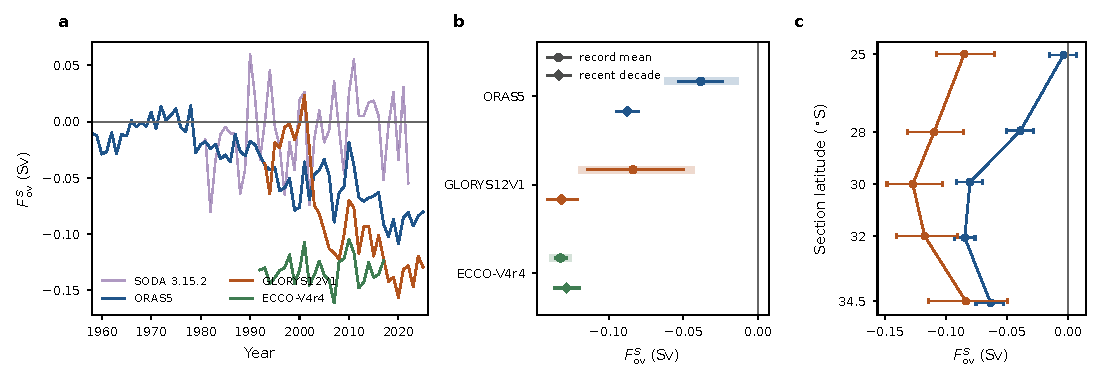
\includegraphics[width=\textwidth]{Fig1_sign.pdf}
  \DIFaddendFL \caption{\DIFdelbeginFL \textbf{\DIFdelFL{Overturning freshwater transport at 34.5\degS{} in four
  ocean reanalyses.}}
  %DIFAUXCMD
\DIFdelendFL \DIFaddbeginFL \textbf{\DIFaddFL{The sign of the overturning freshwater transport at
  34.5\degS{}.}}
  \DIFaddendFL \textbf{a}, Annual-mean $\Fovs$\DIFdelbeginFL \DIFdelFL{for }\DIFdelendFL \DIFaddbeginFL \DIFaddFL{. }\DIFaddendFL ORAS5\DIFdelbeginFL \DIFdelFL{(1958--2025)}\DIFdelendFL , GLORYS12V1 \DIFdelbeginFL \DIFdelFL{(1993--2025), ECCO-V4r4 (1992--2017) }\DIFdelendFL and \DIFaddbeginFL \DIFaddFL{ECCO-V4r4 are computed
  here from monthly fields on the contiguous Atlantic section; }\DIFaddendFL SODA 3.15.2 \DIFdelbeginFL \DIFdelFL{(1980--2022);
  horizontal lines mark each record mean}\DIFdelendFL \DIFaddbeginFL \DIFaddFL{is
  carried over from an annual-field pipeline, is not on the same basis, and is
  not used in any quantitative claim}\DIFaddendFL .
  \textbf{b}, Record \DIFdelbeginFL \DIFdelFL{means }\DIFdelendFL \DIFaddbeginFL \DIFaddFL{mean (circles) and most recent decade (diamonds) }\DIFaddendFL with 95\%
  circular block-bootstrap \DIFdelbeginFL \DIFdelFL{confidence
  }\DIFdelendFL intervals\DIFdelbeginFL \DIFdelFL{(}\DIFdelendFL \DIFaddbeginFL \DIFaddFL{, at a }\DIFaddendFL 5-year \DIFdelbeginFL \DIFdelFL{blocks}\DIFdelendFL \DIFaddbeginFL \DIFaddFL{block for the record mean and
  a 3-year block for the decade. The pale bar spans the intervals obtained for
  block lengths of 2 to 20 years. Between-product spread is 0.094~Sv}\DIFaddendFL , \DIFdelbeginFL \DIFdelFL{10}%DIFDELCMD < {%%%
\DIFdelendFL \DIFaddbeginFL \DIFaddFL{wider than
  the widest of these intervals (0.073~Sv}\DIFaddendFL , \DIFdelbeginFL %DIFDELCMD < }%%%
\DIFdelFL{000 iterations}\DIFdelendFL \DIFaddbeginFL \DIFaddFL{GLORYS12V1 across block lengths}\DIFaddendFL ) \DIFdelbeginFL \DIFdelFL{; solid }\DIFdelendFL \DIFaddbeginFL \DIFaddFL{and
  1.5 times the 5-year }\DIFaddendFL intervals \DIFdelbeginFL \DIFdelFL{exclude zero,
  dashed do not}\DIFdelendFL \DIFaddbeginFL \DIFaddFL{quoted in the text}\DIFaddendFL .
  \textbf{c}, \DIFaddbeginFL \DIFaddFL{Mean }\DIFaddendFL $\Fovs$ \DIFdelbeginFL \DIFdelFL{trends over each product's own record (circles) and }\DIFdelendFL over \DIFaddbeginFL \DIFaddFL{1993--2025 against section latitude, with }\DIFaddendFL the
  \DIFdelbeginFL \DIFdelFL{common 1993--2017 window (diamonds). Filled markers indicate a
  Santer-adjusted $p<0.05$}\DIFdelendFL \DIFaddbeginFL \DIFaddFL{same intervals}\DIFaddendFL . \DIFdelbeginFL \DIFdelFL{No product has a significant trend in }\DIFdelendFL \DIFaddbeginFL \DIFaddFL{The open marker is }\DIFaddendFL the \DIFdelbeginFL \DIFdelFL{common
  window}\DIFdelendFL \DIFaddbeginFL \DIFaddFL{one case whose interval includes zero}\DIFaddendFL .}
  \DIFdelbeginFL %DIFDELCMD < \label{fig:regime}
%DIFDELCMD < %%%
\DIFdelendFL \DIFaddbeginFL \label{fig:sign}
\DIFaddendFL \end{figure}

\begin{figure}[t]
  \centering
  \DIFdelbeginFL %DIFDELCMD < \includegraphics[width=\textwidth]{Fig2_mechanism.pdf}
%DIFDELCMD <   %%%
\DIFdelendFL \DIFaddbeginFL 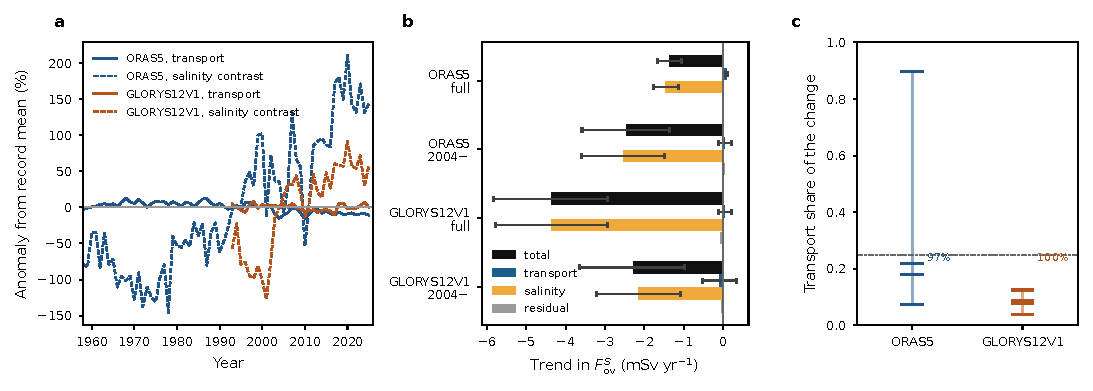
\includegraphics[width=\textwidth]{Fig2_attribution.pdf}
  \DIFaddendFL \caption{\DIFdelbeginFL \textbf{\DIFdelFL{The decline in $\Fovs$ is not a change in overturning
  strength.}}
  %DIFAUXCMD
\DIFdelendFL \DIFaddbeginFL \textbf{\DIFaddFL{The decline is carried by the salinity contrast, not by the
  transport.}}
  \DIFaddendFL \textbf{a}, \DIFdelbeginFL \DIFdelFL{Annual upper-cell overturning strength at the 34.5\degS{}
  section}\DIFdelendFL \DIFaddbeginFL \DIFaddFL{The two factors of equation~\eqref{eq:factorisation}}\DIFaddendFL , \DIFdelbeginFL \DIFdelFL{computed on the same grid row }\DIFdelendFL \DIFaddbeginFL \DIFaddFL{each }\DIFaddendFL as \DIFdelbeginFL \DIFdelFL{$\Fovs$}\DIFdelendFL \DIFaddbeginFL \DIFaddFL{a
  percentage anomaly from its own record mean}\DIFaddendFL , \DIFaddbeginFL \DIFaddFL{so that a factor which barely
  moves can be compared }\DIFaddendFL with \DIFdelbeginFL \DIFdelFL{least-squares trends
  (solid where }\DIFdelendFL \DIFaddbeginFL \DIFaddFL{one that moves a great deal. The ORAS5 contrast
  passes close to zero early in }\DIFaddendFL the \DIFdelbeginFL \DIFdelFL{Santer-adjusted $p<0.05$}\DIFdelendFL \DIFaddbeginFL \DIFaddFL{record}\DIFaddendFL , \DIFdelbeginFL \DIFdelFL{dashed otherwise)}\DIFdelendFL \DIFaddbeginFL \DIFaddFL{which is why its percentage anomaly
  is large there}\DIFaddendFL .
  \textbf{b}, \DIFdelbeginFL \DIFdelFL{The three terms of equation~\eqref{eq:identity} for four
  early-to-late epoch pairs; the black tick marks the total change. The
  overturning term is small }\DIFdelendFL \DIFaddbeginFL \DIFaddFL{Trend }\DIFaddendFL in \DIFdelbeginFL \DIFdelFL{every case }\DIFdelendFL \DIFaddbeginFL \DIFaddFL{$\Fovs$ split into transport and salinity contributions
  with 95\% block-bootstrap intervals, }\DIFaddendFL and \DIFdelbeginFL \DIFdelFL{mostly opposes }\DIFdelendFL the \DIFdelbeginFL \DIFdelFL{total}\DIFdelendFL \DIFaddbeginFL \DIFaddFL{covariance residual, over each
  product's own record and over the Argo era}\DIFaddendFL .
  \textbf{c}, \DIFdelbeginFL \DIFdelFL{The same }\DIFdelendFL \DIFaddbeginFL \DIFaddFL{Transport share of the change over every non-overlapping }\DIFaddendFL epoch
  \DIFdelbeginFL \DIFdelFL{pairs decomposed on }\DIFdelendFL \DIFaddbeginFL \DIFaddFL{pair }\DIFaddendFL the \DIFdelbeginFL \DIFdelFL{full depth profile into
  velocity}\DIFdelendFL \DIFaddbeginFL \DIFaddFL{record supports (2901 for ORAS5}\DIFaddendFL , \DIFdelbeginFL \DIFdelFL{salinity }\DIFdelendFL \DIFaddbeginFL \DIFaddFL{151 for GLORYS12V1) at epoch lengths
  of 10, 13 }\DIFaddendFL and \DIFdelbeginFL \DIFdelFL{cross terms}\DIFdelendFL \DIFaddbeginFL \DIFaddFL{15 years, treated as a sensitivity analysis over window choice}\DIFaddendFL .
  \DIFdelbeginFL \DIFdelFL{The hatched segment is the part of }\DIFdelendFL \DIFaddbeginFL \DIFaddFL{Ticks mark }\DIFaddendFL the \DIFdelbeginFL \DIFdelFL{velocity term explained by rescaling }\DIFdelendFL \DIFaddbeginFL \DIFaddFL{median, 90th and 95th percentiles and }\DIFaddendFL the \DIFdelbeginFL \DIFdelFL{overturning}\DIFdelendFL \DIFaddbeginFL \DIFaddFL{maximum}\DIFaddendFL ; the
  \DIFdelbeginFL \DIFdelFL{remainder }\DIFdelendFL \DIFaddbeginFL \DIFaddFL{percentage }\DIFaddendFL is \DIFdelbeginFL \DIFdelFL{a
  change in its vertical structure}\DIFdelendFL \DIFaddbeginFL \DIFaddFL{the fraction of pairs below the dashed 0.25 line}\DIFaddendFL .}
  \DIFdelbeginFL %DIFDELCMD < \label{fig:mechanism}
%DIFDELCMD < %%%
\DIFdelendFL \DIFaddbeginFL \label{fig:attribution}
\DIFaddendFL \end{figure}

\begin{figure}[t]
  \centering
  \DIFdelbeginFL %DIFDELCMD < \includegraphics[width=\textwidth]{Fig3_saltredist.pdf}
%DIFDELCMD <   %%%
\DIFdelendFL \DIFaddbeginFL 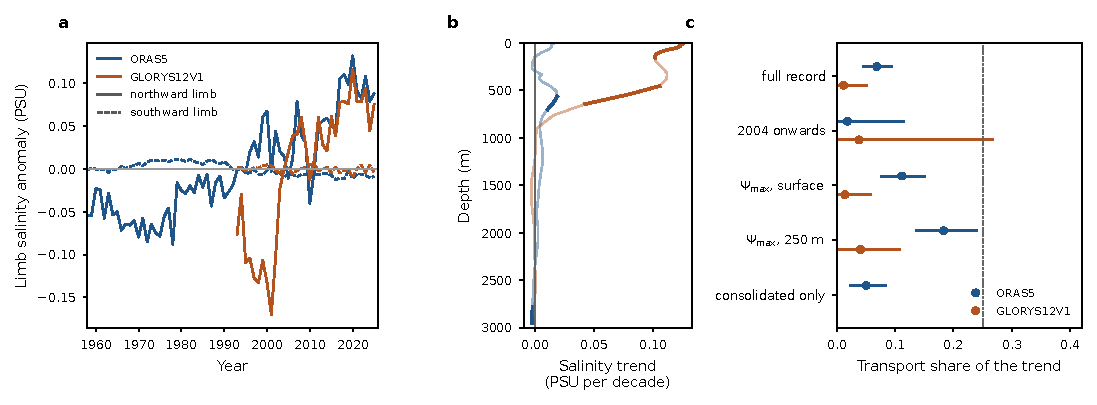
\includegraphics[width=\textwidth]{Fig3_mechanism.pdf}
  \DIFaddendFL \caption{\DIFdelbeginFL \textbf{\DIFdelFL{Salinity change at and around the section, and where the two
  eddy-permitting products disagree.}}
  %DIFAUXCMD
\DIFdelendFL \DIFaddbeginFL \textbf{\DIFaddFL{The northward limb salinifies; the southward limb does not.}}
  \DIFaddendFL \textbf{a}, \DIFdelbeginFL \DIFdelFL{Interbasin surface }\DIFdelendFL \DIFaddbeginFL \DIFaddFL{Transport-weighted }\DIFaddendFL salinity \DIFdelbeginFL \DIFdelFL{contrast, subtropical South Atlantic
  minus subtropical South Indo-Pacific, over 1993--2024, with least-squares
  trends. The Indo-Pacific box is wrapped across }\DIFdelendFL \DIFaddbeginFL \DIFaddFL{of }\DIFaddendFL the \DIFdelbeginFL \DIFdelFL{date line}\DIFdelendFL \DIFaddbeginFL \DIFaddFL{northward limb (solid) and the
  southward limb (dashed), as anomalies from their record means}\DIFaddendFL .
  \textbf{b}, Zonal-mean salinity trend against depth at the \DIFdelbeginFL \DIFdelFL{34.5\degS{}
  }\DIFdelendFL section over
  1993--2025, \DIFdelbeginFL \DIFdelFL{on colour-matched axes with a common zero because
  the two products differ by a factor of about 29 in the upper layer. Solid
  }\DIFdelendFL \DIFaddbeginFL \DIFaddFL{drawn bold }\DIFaddendFL where the \DIFaddbeginFL \DIFaddFL{pointwise }\DIFaddendFL Santer-adjusted \DIFdelbeginFL \DIFdelFL{$p<0.05$}\DIFdelendFL \DIFaddbeginFL \DIFaddFL{$p$ is below 0.05}\DIFaddendFL .
  \DIFdelbeginFL \textbf{\DIFdelFL{c}}%DIFAUXCMD
\DIFdelFL{, Vertical salinity contrast }\DIFdelendFL \DIFaddbeginFL \DIFaddFL{The panel is truncated }\DIFaddendFL at \DIFdelbeginFL \DIFdelFL{the section, upper limb
  (0 to 1000}\DIFdelendFL \DIFaddbeginFL \DIFaddFL{3000}\DIFaddendFL ~m\DIFdelbeginFL \DIFdelFL{) minus deep }\DIFdelendFL \DIFaddbeginFL \DIFaddFL{; the abyssal }\DIFaddendFL limb \DIFdelbeginFL \DIFdelFL{(1000 to 3000}\DIFdelendFL \DIFaddbeginFL \DIFaddFL{discussed in the text
  begins below 4000}\DIFaddendFL ~m\DIFdelbeginFL \DIFdelFL{)}\DIFdelendFL \DIFaddbeginFL \DIFaddFL{.
  Adjacent levels are strongly correlated}\DIFaddendFL , \DIFdelbeginFL \DIFdelFL{with least-squares trends
  drawn solid where }\DIFdelendFL \DIFaddbeginFL \DIFaddFL{so no field-significance claim is
  made from this panel.
  }\textbf{\DIFaddFL{c}}\DIFaddFL{, Transport share of }\DIFaddendFL the \DIFdelbeginFL \DIFdelFL{Santer-adjusted $p<0.05$; neither reaches that
  threshold over }\DIFdelendFL \DIFaddbeginFL \DIFaddFL{$\Fovs$ trend under every robustness test,
  with 95\% block-bootstrap intervals: }\DIFaddendFL the full \DIFdelbeginFL \DIFdelFL{window. This is }\DIFdelendFL \DIFaddbeginFL \DIFaddFL{record, }\DIFaddendFL the \DIFdelbeginFL \DIFdelFL{quantity that enters
  equation~\eqref{eq:identity}. Its trend is an order }\DIFdelendFL \DIFaddbeginFL \DIFaddFL{Argo era, two
  alternative definitions }\DIFaddendFL of \DIFdelbeginFL \DIFdelFL{magnitude larger in
  GLORYS12V1 ($+0.071$~PSU per decade}\DIFdelendFL \DIFaddbeginFL \DIFaddFL{the overturning strength}\DIFaddendFL , \DIFdelbeginFL \DIFdelFL{$p=0.08$) than in }\DIFdelendFL \DIFaddbeginFL \DIFaddFL{and, for }\DIFaddendFL ORAS5\DIFdelbeginFL \DIFdelFL{($+0.006$}\DIFdelendFL , \DIFdelbeginFL \DIFdelFL{$p=0.80$)}\DIFdelendFL \DIFaddbeginFL \DIFaddFL{the
  homogeneous consolidated stream alone}\DIFaddendFL .}
  \DIFdelbeginFL %DIFDELCMD < \label{fig:saltredist}
%DIFDELCMD < %%%
\DIFdelendFL \DIFaddbeginFL \label{fig:mechanism}
\DIFaddendFL \end{figure}

\begin{figure}[t]
  \centering
  \DIFdelbeginFL %DIFDELCMD < \includegraphics[width=\textwidth]{Fig4_cmip6.pdf}
%DIFDELCMD <   %%%
\DIFdelendFL \DIFaddbeginFL 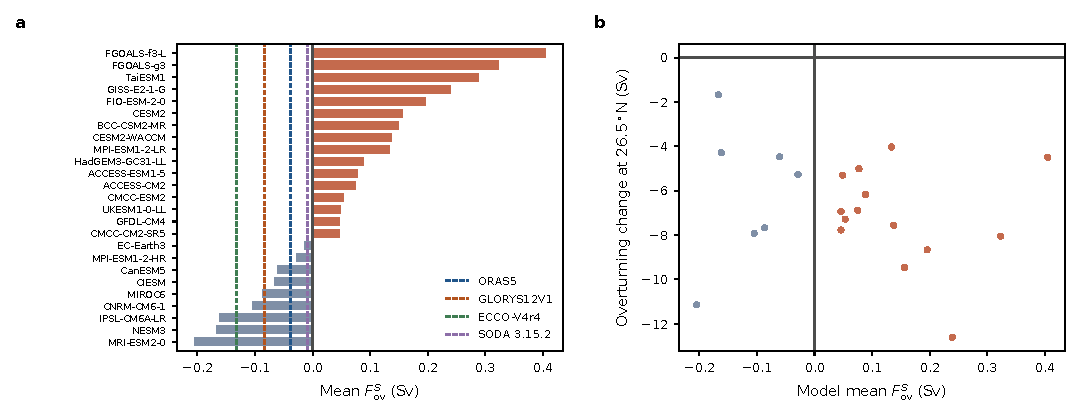
\includegraphics[width=\textwidth]{Fig4_models.pdf}
  \DIFaddendFL \caption{\DIFdelbeginFL \textbf{\DIFdelFL{CMIP6 sits on the other side of zero, and the sign does not
  predict the rate.}}
  %DIFAUXCMD
\DIFdelendFL \DIFaddbeginFL \textbf{\DIFaddFL{CMIP6 lies above the observational estimates, but cannot be
  sorted by the sign of $\Fovs$.}}
  \DIFaddendFL \textbf{a}, \DIFdelbeginFL \DIFdelFL{Historical mean }\DIFdelendFL \DIFaddbeginFL \DIFaddFL{Mean }\DIFaddendFL $\Fovs$ at 34.5\degS{} \DIFaddbeginFL \DIFaddFL{over 1950--1980 }\DIFaddendFL in 25 CMIP6 models,
  with the \DIFdelbeginFL \DIFdelFL{four }\DIFdelendFL reanalysis estimates marked; \DIFdelbeginFL \DIFdelFL{16 of 25 }\DIFdelendFL \DIFaddbeginFL \DIFaddFL{SODA is shown for continuity with
  Fig.~\ref{fig:sign} and is not used quantitatively. No offset or bias
  correction is applied to either }\DIFaddendFL models \DIFdelbeginFL \DIFdelFL{are positive}\DIFdelendFL \DIFaddbeginFL \DIFaddFL{or reanalyses}\DIFaddendFL .
  \textbf{b}, Model mean $\Fovs$ against the \DIFdelbeginFL \DIFdelFL{2005--2023 }\DIFdelendFL overturning \DIFdelbeginFL \DIFdelFL{trend }\DIFdelendFL \DIFaddbeginFL \DIFaddFL{change }\DIFaddendFL at 26.5\degN{}
  \DIFdelbeginFL \DIFdelFL{for }\DIFdelendFL \DIFaddbeginFL \DIFaddFL{from 1850--1900 to 2081--2100 in }\DIFaddendFL the \DIFdelbeginFL \DIFdelFL{16 }\DIFdelendFL \DIFaddbeginFL \DIFaddFL{21 }\DIFaddendFL models with \DIFdelbeginFL \DIFdelFL{the required output, with the RAPID,
  ORAS5 and GLORYS12V1 estimates for the same window. The two quantities are
  uncorrelated }\DIFdelendFL \DIFaddbeginFL \DIFaddFL{historical plus ssp585
  projections }\DIFaddendFL (\DIFdelbeginFL \DIFdelFL{Pearson $r=-0.04$}\DIFdelendFL \DIFaddbeginFL \DIFaddFL{$r=-0.20$}\DIFaddendFL , \DIFdelbeginFL \DIFdelFL{$p=0.88$; Spearman $\rho=+0.07$}\DIFdelendFL \DIFaddbeginFL \DIFaddFL{$p=0.40$}\DIFaddendFL , \DIFdelbeginFL \DIFdelFL{$p=0.79$}\DIFdelendFL \DIFaddbeginFL \DIFaddFL{smallest reachable $|r|=0.43$}\DIFaddendFL ). \DIFdelbeginFL \DIFdelFL{Model numbering }\DIFdelendFL \DIFaddbeginFL \DIFaddFL{This
  replaces a 19-year single-member trend test, whose null result }\DIFaddendFL is \DIFdelbeginFL \DIFdelFL{given in Extended Data Table}\DIFdelendFL \DIFaddbeginFL \DIFaddFL{guaranteed
  by internal variability: 19-year trends span $-3.5$ to $+2.4$}\DIFaddendFL ~\DIFdelbeginFL \DIFdelFL{1.}\DIFdelendFL \DIFaddbeginFL \DIFaddFL{Sv per decade
  across 50 members of the MPI-ESM1-2-LR large ensemble.}\DIFaddendFL }
  \DIFdelbeginFL %DIFDELCMD < \label{fig:cmip6}
%DIFDELCMD < %%%
\DIFdelendFL \DIFaddbeginFL \label{fig:models}
\DIFaddendFL \end{figure}

\section*{Discussion}

Two statements about $\Fovs$ have been run together\DIFdelbegin \DIFdel{in the recent literature}\DIFdelend , and they need to be
separated. The first is that the Atlantic freshwater budget at 34.5\degS{} sits
on the side where the salt-advection feedback is self-reinforcing. \DIFdelbegin \DIFdel{Four reanalyses spanning three }\DIFdelend \DIFaddbegin \DIFadd{Three
reanalyses spanning two }\DIFaddend ocean models and \DIFdelbegin \DIFdel{four
assimilation schemes }\DIFdelend \DIFaddbegin \DIFadd{three assimilation methods }\DIFaddend agree on
that, \DIFdelbegin \DIFdel{three of them with confidence }\DIFdelend \DIFaddbegin \DIFadd{with }\DIFaddend intervals clear of zero \DIFdelbegin \DIFdel{, and the result does not
depend on the reference salinity, which rescales every magnitude by $35/S_0$
and leaves the attribution exactly unchanged}\DIFdelend \DIFaddbegin \DIFadd{at every block length we tried, at every
latitude from 28 to 34.5\degS{} in the two products run on the latitude ladder, and in the most recent decade of each record}\DIFaddend .
The second is that the observed decline in $\Fovs$ measures a weakening
overturning. That statement does not survive contact with the same data.

The reason is \DIFdelbegin \DIFdel{structural rather than statistical. With $\Fovs<0$ the overturning-weighted salinity contrast is positive, so a weakening circulation
raises }\DIFdelend \DIFaddbegin \DIFadd{a rate comparison rather than a ratio. In the two products that
decline, }\DIFaddend $\Fovs$ \DIFdelbegin \DIFdel{\mbox{%DIFAUXCMD
\cite{Vanderborght2025}}\hskip0pt%DIFAUXCMD
. Our decomposition shows that this is not
a theoretical caveat but the actual situation: the overturning at 34.5\degS{}
weakens in ORAS5 by 10\% between the two epochs and by 2.9\%in GLORYS12V1}\DIFdelend \DIFaddbegin \DIFadd{is changing at 36\% and 52\% of its own magnitude per decade
while the volume transport that carries it changes at 2.6\% and 0.6\%. Passed
through equation~\eqref{eq:factorisation} this makes the transport contribution
between 1\% and 18\% of the trend depending on how the overturning is defined
and over which window, with individual intervals reaching 27\%}\DIFaddend , and in \DIFdelbegin \DIFdel{both cases that weakening pushes $\Fovs$ upward while the observed
change is downward. Whatever the recent decline in $\Fovs$ records, }\DIFdelend \DIFaddbegin \DIFadd{most
configurations it has the opposite sign to the total. It is a minority
contribution under every test we ran in which the share is identified, though }\DIFaddend it
is not \DIFdelbegin \DIFdel{the overturning slowing down}\DIFdelend \DIFaddbegin \DIFadd{definition-independent:
it rises systematically as the definition of the overturning narrows from the
whole northward limb to the streamfunction maximum}\DIFaddend . Studies that read a falling
$\Fovs$ as a proxy for AMOC weakening, including \DIFdelbegin \DIFdel{our own earlier work, have }\DIFdelend the \DIFdelbegin \DIFdel{sign of the leading term backwards}\DIFdelend \DIFaddbegin \DIFadd{early-warning arguments
built on the $\Fovs$ minimum\mbox{%DIFAUXCMD
\cite{vanWesten2024} }\hskip0pt%DIFAUXCMD
and an earlier, unpublished
version of our own analysis of these data, have attributed to the circulation a
change that the circulation did not make}\DIFaddend .

\DIFdelbegin \DIFdel{We are also careful about what the negative sign licenses. A negative }\DIFdelend \DIFaddbegin \DIFadd{What did make it is a widening of the salinity contrast between the limbs,
carried by the northward limb while the southward limb does not change. How much
of that is a water-mass change rather than a redistribution of transport in
depth differs between products: in GLORYS12V1 it is 94\%, in ORAS5 only about
two thirds, with the salinity-only part there not individually significant. The
coarse upper-to-abyssal redistribution is small in both, and excluding the
abyssal cell makes the salinification larger rather than smaller, so what
remains in ORAS5 is a rearrangement of transport within the upper limb.
}

\DIFadd{The part of this that observations can check, they support. Holding the
circulation fixed and letting only the EN4 objective analysis vary, the
northward limb salinifies at $+0.026$ to $+0.028$~PSU per decade
($p\le0.0005$) while the southward limb is flat. The limb asymmetry is
therefore present in a salinity field that no model integrates forward, and the
same construction returns a negative }\DIFaddend $\Fovs$\DIFdelbegin \DIFdel{identifies a regime in
which multiple equilibria are permitted in the class of
models where the diagnostic was developed\mbox{%DIFAUXCMD
\cite{deVries2005,Huisman2010}}\hskip0pt%DIFAUXCMD
. It is not a measurement of bistability in the real ocean.
Box models with a more
complete treatment of the northern boundary\mbox{%DIFAUXCMD
\cite{Cimatoribus2014} }\hskip0pt%DIFAUXCMD
and hysteresis
experiments in a modern coupled model \mbox{%DIFAUXCMD
\cite{vanWestenDijkstra2023} }\hskip0pt%DIFAUXCMD
both show that the collapsed branch can exist outside the $\Fovs<0$ range, so the sign locates the freshwater budget rather than proving that a second state is reachable. The same literature cautions that }\DIFdelend \DIFaddbegin \DIFadd{, $-0.080$ to $-0.128$~Sv, from
observed salinity. The rate is less secure: ORAS5 runs about twice the
observation-only value over the same years while GLORYS12V1 is within 30\% of
it, and part of that gap is expected because EN4 relaxes to climatology where
profiles are sparse. The direction should be trusted; the ORAS5 rate should
not.
It also reframes what the diagnostic is sensing. A salinifying upper limb widens
the limb contrast and drives $\Fovs$ downward regardless of what the overturning
does, which is why $\Fovs$ and the transport are so weakly coupled on the
timescales the records resolve. It is consistent in direction with the South
Atlantic salinity accumulation attributed to a weakening
overturning\mbox{%DIFAUXCMD
\cite{Zhu2020,Zhu2023}}\hskip0pt%DIFAUXCMD
, but our decomposition locates the change in
the transport-weighted upper limb rather than in the surface field, and we find
no transport change to accompany it.
}

\DIFadd{Two things temper this. The first is that $\Fovs$ is not the freshwater budget
of the basin. The azonal component at this section is several times larger, of
the opposite sign, and trending upward by more than }\DIFaddend $\Fovs$ is \DIFdelbegin \DIFdel{a quasi-equilibrium
diagnostic\mbox{%DIFAUXCMD
\cite{Liu2017}}\hskip0pt%DIFAUXCMD
, informative about sensitivity to forcing but limited
as a transient indicator, because northern
salinity anomalies take decades to
reach the southern boundary and an AMOC collapse in a coupled model need not coincide with a minimum in }\DIFdelend \DIFaddbegin \DIFadd{trending
downward: significantly so in ORAS5, and marginally in GLORYS12V1 ($p=0.049$ on
8.5 effective degrees of freedom). Whether the basin as a whole is
moving deeper into the self-reinforcing regime is therefore not settled by
}\DIFaddend $\Fovs$ \DIFdelbegin \DIFdel{\mbox{%DIFAUXCMD
\cite{vanWesten2025}}\hskip0pt%DIFAUXCMD
. Our results are an
observational counterpart to that caution}\DIFdelend \DIFaddbegin \DIFadd{alone, and we make no claim that it is. Nor do we evaluate the northern
boundary: the indicator in the theory we cite is the freshwater convergence
between the southern and northern boundaries, and $\Fovs$ is a proxy for it
whose adequacy we have not tested. Both are natural next steps and neither is
addressed here}\DIFaddend .

The \DIFdelbegin \DIFdel{disagreement between the two eddy-permitting products is worth stating
plainly rather than averaging away.
}\DIFdelend \DIFaddbegin \DIFadd{second is ECCO-V4r4, and it is a genuine disagreement rather than a caveat.
It is the only product here that is dynamically consistent by construction and
therefore the only one whose freshwater budget closes without assimilation
increments, and it shows no decline in $\Fovs$. Its limb salinities are flat only in the
aggregate: its upper cell salinifies at $+0.022$~PSU per decade ($p=0.025$),
the same sign as the other two products, while a significant redistribution
towards its abyssal cell cancels the effect. Against }\DIFaddend GLORYS12V1 \DIFdelbegin \DIFdel{puts the change in the
salinity
field at the section, with an upper-layer trend of $+0.109$}\DIFdelend \DIFaddbegin \DIFadd{this is
not an underpowered null: on the window the two share, ECCO's minimum detectable
limb-salinity trend of 0.020}\DIFaddend ~PSU per decade \DIFdelbegin \DIFdel{;
ORAS5 puts it in the vertical structure of
the flow, with an upper-layer
salinity trend 29 times smaller. Both use NEMO and ERA-family forcing, so this
is a disagreement between two closely related systems, and it bounds how much
confidence any single-product mechanism claim deserves.
It is also a reminder
that the reanalyses are least constrained by observations exactly where we
evaluate them: the observing network at 34.5\degS{} is
far sparser than }\DIFdelend \DIFaddbegin \DIFadd{is well below the GLORYS12V1 rate of
$+0.083$, so ECCO could have seen that salinification and did not. Against
ORAS5, whose common-window rate is $+0.019$, the comparison is inconclusive.
ECCO is also }\DIFaddend the \DIFdelbegin \DIFdel{sustained array at 26.5\degN{}\mbox{%DIFAUXCMD
\cite{Meinen2018,Cunningham2007}}\hskip0pt%DIFAUXCMD
, and the SAMBA
occupation is too short to arbitrate\mbox{%DIFAUXCMD
\cite{FrajkaWilliams2019}}\hskip0pt%DIFAUXCMD
.
}%DIFDELCMD < 

%DIFDELCMD < %%%
\DIFdel{For models the implication cuts two ways. Correcting the freshwater transport
bias is necessary if a
model is to represent the salt-advection feedback at
all,
and two thirds of CMIP6 currently cannot. But the same models show no
relationship between the sign of $\Fovs$ and the rate at which their
overturning weakens,
so a bias correction of this kind should not be expected
to sharpen projections of the rate. The two properties are logically
independent, and our observational result makes the same point from the other
direction: a basin can sit in the self-reinforcing regime and still change
slowly}\DIFdelend \DIFaddbegin \DIFadd{one product in which the coarse limb redistribution is
significant and acts to cancel a positive water-mass term, so its flat limb
salinity is a cancellation rather than an absence of change. The mechanism we report is therefore a
property of the two sequential-assimilation products, and it remains possible
that what they are tracking is the arrival of the Argo array rather than a
change in the ocean. The evidence against that reading is that the attribution
is unchanged in every window and under every inhomogeneity correction we tried,
and that EN4 reproduces the limb asymmetry independently. The evidence for it is
that both sequential-assimilation products step at an observing-system boundary:
GLORYS12V1's decline is a level shift at the 2004 Argo transition rather than a
trend, and the ORAS5 record steps across its consolidated-to-operational join,
significantly so in the limb salinity itself ($+0.038$~PSU, $p=0.029$), after
which its Argo-era trend is no longer significant. Neither product's }\emph{\DIFadd{rate}}
\DIFadd{of decline should be taken at face value. We could not obtain the salinity
assimilation increments that would settle the question directly, and we regard
it as open}\DIFaddend .

\DIFdelbegin \DIFdel{Several limitations bound these conclusions. All four reanalyses }\DIFdelend \DIFaddbegin \DIFadd{Beyond that, all of these products }\DIFaddend are forced by the ERA family, \DIFdelbegin \DIFdel{ORAS5 and GLORYS12V1 by ERA-Interim and ERA5, ECCO-V4r4 by
adjusted ERA-Interim and SODA 3.15.2 by ERA5, and all of them assimilate
overlapping observations. Cross-product agreement is therefore }\DIFdelend \DIFaddbegin \DIFadd{so
cross-product agreement is }\DIFaddend a weaker form of independence than the product count
suggests: \DIFdelbegin \DIFdel{the four }\DIFdelend \DIFaddbegin \DIFadd{they }\DIFaddend differ in ocean model and in assimilation scheme, but not in the
atmosphere driving them. The Copernicus distribution of ORAS5 publishes \DIFdelbegin \DIFdel{only
}\DIFdelend one of
the system's five ensemble members\cite{Zuo2019}, so cross-product spread has to
stand in for within-product spread throughout\DIFdelbegin \DIFdel{. The interbasin
index is a surface diagnostic and , as we
show, has no interannual relationship with }\DIFdelend \DIFaddbegin \DIFadd{, and that spread, 0.094~Sv, exceeds even the
widest within-product interval\mbox{%DIFAUXCMD
\cite{Jackson2019}}\hskip0pt%DIFAUXCMD
. We compute
ECCO on the distributed 0.5\degree{} interpolation rather than the native LLC90
grid, which does not conserve transport exactly, and since ECCO is now the
load-bearing counterexample that limitation matters more than it would if it
were one supporting vote among four. The three products differ by 46\% in northward-limb transport
at this section (14.6 to 21.3~Sv), and we have not applied a published SAMBA or
SAMOC mean to arbitrate between them. That omission is not neutral: the weakest
of the three is ECCO, which is also our counterexample, so a comparison against
the observed mean transport could as easily undermine the counterexample as
support it, and it should be done before these numbers are used to weigh one
product against another. The reanalyses are also least
constrained by observations exactly where we evaluate them, since the observing
network at 34.5\degS{} is far sparser than the sustained array at
26.5\degN{}\mbox{%DIFAUXCMD
\cite{Meinen2018,Cunningham2007,GarzoliMatano2011,FrajkaWilliams2019}}\hskip0pt%DIFAUXCMD
.
}

\DIFadd{For models the implication cuts two ways. Correcting the freshwater transport
bias is necessary if a model is to represent the salt-advection feedback with
the right sign, and the CMIP6 median sits above every observational estimate we
computed. But the majority count usually quoted is not distinguishable from a
coin flip once model genealogy is accounted for, and we find no detectable
relationship between the sign of }\DIFaddend $\Fovs$ \DIFdelbegin \DIFdel{once the shared trend is removed; we report it as a description of
the surface salinity field, not as evidence of a mechanism. Surface salinity
trend patterns are in any case ambiguous, since amplification of the water
cycle and a uniform surface heat flux both produce patterns resembling the one
attributed here to ocean transport\mbox{%DIFAUXCMD
\cite{Zika2018}}\hskip0pt%DIFAUXCMD
, which is why the argument
rests on the section decomposition rather than on maps}\DIFdelend \DIFaddbegin \DIFadd{and the rate at which a model's
overturning weakens, either over the satellite era or over the forced response
to 2100, with a sample that could not have detected a moderate one. What we do
find is that model $\Fovs$ is strongly correlated with pre-industrial
overturning strength, which suggests that the freshwater transport bias is
partly a symptom of the overturning strength bias. If that is right, correcting
$\Fovs$ in isolation is the wrong target, and the two biases should be
addressed together}\DIFaddend .

What would settle the \DIFdelbegin \DIFdel{rate }\DIFdelend \DIFaddbegin \DIFadd{transient }\DIFaddend question is observational rather than
analytical. \DIFaddbegin \DIFadd{The claim we make is now a claim about limb salinities, which
sustained hydrography at 34.5\degS{} and the repeat sections that cross it can
test directly, without passing through an assimilating model; projecting an
observation-only salinity analysis onto the same limb mask is the single most
informative next step and we regard it as the test this result should be judged
by. }\DIFaddend Sustained transport monitoring at \DIFdelbegin \DIFdel{34.5\degS{}}\DIFdelend \DIFaddbegin \DIFadd{this latitude}\DIFaddend , extended towards the length
RAPID has reached at 26.5\degN{}, would constrain both factors \DIFdelbegin \DIFdel{in
equation~\eqref{eq:identity} directly instead of through assimilating models}\DIFdelend \DIFaddbegin \DIFadd{of
equation~\eqref{eq:factorisation} at once}\DIFaddend . Reanalyses forced outside the ERA
family would test how much of the present agreement comes from shared boundary
conditions, and release of all five ORAS5 ensemble members would separate
assimilation noise from ocean signal within a single product. Until then the
defensible statement is the narrow one: the Atlantic freshwater budget sits
where the salt-advection feedback is self-reinforcing, and \DIFdelbegin \DIFdel{the trend }\DIFdelend \DIFaddbegin \DIFadd{in the products that
decline, the recent decline }\DIFaddend in that diagnostic \DIFdelbegin \DIFdel{tells us little about how
fast the circulationis changing}\DIFdelend \DIFaddbegin \DIFadd{records a salinifying upper limb
rather than a slowing circulation}\DIFaddend .


\bibliographystyle{naturemag}
\begin{thebibliography}{10}
\expandafter\ifx\csname url\endcsname\relax
  \def\url#1{\texttt{#1}}\fi
\expandafter\ifx\csname urlprefix\endcsname\relax\def\urlprefix{URL }\fi
\providecommand{\bibinfo}[2]{#2}
\providecommand{\eprint}[2][]{\url{#2}}

\bibitem{Stommel1961}
\bibinfo{author}{Stommel, H.}
\newblock \bibinfo{title}{Thermohaline convection with two stable regimes of
  flow}.
\newblock \emph{\bibinfo{journal}{Tellus}} \textbf{\bibinfo{volume}{13}},
  \bibinfo{pages}{224--230} (\bibinfo{year}{1961}).

\bibitem{Rahmstorf1996}
\bibinfo{author}{Rahmstorf, S.}
\newblock \bibinfo{title}{On the freshwater forcing and transport of the
  {Atlantic} thermohaline circulation}.
\newblock \emph{\bibinfo{journal}{Climate Dynamics}}
  \textbf{\bibinfo{volume}{12}}, \bibinfo{pages}{799--811}
  (\bibinfo{year}{1996}).

\bibitem{Rahmstorf2002}
\bibinfo{author}{Rahmstorf, S.}
\newblock \bibinfo{title}{Ocean circulation and climate during the past 120,000
  years}.
\newblock \emph{\bibinfo{journal}{Nature}} \textbf{\bibinfo{volume}{419}},
  \bibinfo{pages}{207--214} (\bibinfo{year}{2002}).

\bibitem{deVries2005}
\bibinfo{author}{de~Vries, P.} \& \bibinfo{author}{Weber, S.~L.}
\newblock \bibinfo{title}{The {Atlantic} freshwater budget as a diagnostic for
  the existence of a stable shut down of the {North Atlantic} overturning
  circulation}.
\newblock \emph{\bibinfo{journal}{Geophysical Research Letters}}
  \textbf{\bibinfo{volume}{32}}, \bibinfo{pages}{L09606}
  (\bibinfo{year}{2005}).

\bibitem{Huisman2010}
\bibinfo{author}{Huisman, S.~E.}, \bibinfo{author}{den Toom, M.},
  \bibinfo{author}{Dijkstra, H.~A.} \& \bibinfo{author}{Drijfhout, S.}
\newblock \bibinfo{title}{An indicator of the multiple equilibria regime of the
  {Atlantic Meridional Overturning Circulation}}.
\newblock \emph{\bibinfo{journal}{Journal of Physical Oceanography}}
  \textbf{\bibinfo{volume}{40}}, \bibinfo{pages}{551--567}
  (\bibinfo{year}{2010}).

\bibitem{Dijkstra2007}
\bibinfo{author}{Dijkstra, H.~A.}
\newblock \bibinfo{title}{Characterization of the multiple equilibria regime in
  a global ocean model}.
\newblock \emph{\bibinfo{journal}{Tellus A: Dynamic Meteorology and
  Oceanography}} \textbf{\bibinfo{volume}{59}}, \bibinfo{pages}{695--705}
  (\bibinfo{year}{2007}).

\bibitem{Weijer2019}
\bibinfo{author}{Weijer, W.} \emph{et~al.}
\newblock \bibinfo{title}{Stability of the {Atlantic Meridional Overturning
  Circulation}: A review and synthesis}.
\newblock \emph{\bibinfo{journal}{Journal of Geophysical Research: Oceans}}
  \textbf{\bibinfo{volume}{124}}, \bibinfo{pages}{5336--5375}
  (\bibinfo{year}{2019}).

\bibitem{Mecking2017}
\bibinfo{author}{Mecking, J.~V.}, \bibinfo{author}{Drijfhout, S.~S.},
  \bibinfo{author}{Jackson, L.~C.} \& \bibinfo{author}{Andrews, M.~B.}
\newblock \bibinfo{title}{The effect of model bias on {Atlantic} freshwater
  transport and implications for {AMOC} bi-stability}.
\newblock \emph{\bibinfo{journal}{Tellus A: Dynamic Meteorology and
  Oceanography}} \textbf{\bibinfo{volume}{69}}, \bibinfo{pages}{1299910}
  (\bibinfo{year}{2017}).

\bibitem{vanWestenDijkstra2024}
\bibinfo{author}{van Westen, R.~M.} \& \bibinfo{author}{Dijkstra, H.~A.}
\newblock \bibinfo{title}{Persistent climate model biases in the {Atlantic
  Ocean}'s freshwater transport}.
\newblock \emph{\bibinfo{journal}{Ocean Science}}
  \textbf{\bibinfo{volume}{20}}, \bibinfo{pages}{549--567}
  (\bibinfo{year}{2024}).

\bibitem{Cimatoribus2014}
\bibinfo{author}{Cimatoribus, A.~A.}, \bibinfo{author}{Drijfhout, S.~S.} \&
  \bibinfo{author}{Dijkstra, H.~A.}
\newblock \bibinfo{title}{Meridional overturning circulation: stability and
  ocean feedbacks in a box model}.
\newblock \emph{\bibinfo{journal}{Climate Dynamics}}
  \textbf{\bibinfo{volume}{42}}, \bibinfo{pages}{311--328}
  (\bibinfo{year}{2014}).

\bibitem{vanWestenDijkstra2023}
\bibinfo{author}{van Westen, R.~M.} \& \bibinfo{author}{Dijkstra, H.~A.}
\newblock \bibinfo{title}{Asymmetry of {AMOC} hysteresis in a state-of-the-art
  global climate model}.
\newblock \emph{\bibinfo{journal}{Geophysical Research Letters}}
  \textbf{\bibinfo{volume}{50}}, \bibinfo{pages}{e2023GL106088}
  (\bibinfo{year}{2023}).

\bibitem{vanWesten2025}
\bibinfo{author}{van Westen, R.~M.}, \bibinfo{author}{Vanderborght, E.},
  \bibinfo{author}{Kliphuis, M.} \& \bibinfo{author}{Dijkstra, H.~A.}
\newblock \bibinfo{title}{Physics-based indicators for the onset of an {AMOC}
  collapse under climate change}.
\newblock \emph{\bibinfo{journal}{Journal of Geophysical Research: Oceans}}
  \textbf{\bibinfo{volume}{130}}, \bibinfo{pages}{e2025JC022651}
  (\bibinfo{year}{2025}).

\bibitem{Vanderborght2025}
\bibinfo{author}{Vanderborght, E.}, \bibinfo{author}{van Westen, R.~M.} \&
  \bibinfo{author}{Dijkstra, H.~A.}
\newblock \bibinfo{title}{Feedback processes causing an {AMOC} collapse in the
  {Community Earth System Model}}.
\newblock \emph{\bibinfo{journal}{Journal of Climate}}  (\bibinfo{year}{2025}).

\bibitem{vanWesten2024}
\bibinfo{author}{van Westen, R.~M.}, \bibinfo{author}{Kliphuis, M.} \&
  \bibinfo{author}{Dijkstra, H.~A.}
\newblock \bibinfo{title}{Physics-based early warning signal shows that {AMOC}
  is on tipping course}.
\newblock \emph{\bibinfo{journal}{Science Advances}}
  \textbf{\bibinfo{volume}{10}}, \bibinfo{pages}{eadk1189}
  (\bibinfo{year}{2024}).

\bibitem{Zhu2020}
\bibinfo{author}{Zhu, C.} \& \bibinfo{author}{Liu, Z.}
\newblock \bibinfo{title}{Weakening {Atlantic} overturning circulation causes
  {South Atlantic} salinity pile-up}.
\newblock \emph{\bibinfo{journal}{Nature Climate Change}}
  \textbf{\bibinfo{volume}{10}}, \bibinfo{pages}{998--1003}
  (\bibinfo{year}{2020}).

\bibitem{Zhu2023}
\bibinfo{author}{Zhu, C.}, \bibinfo{author}{Liu, Z.}, \bibinfo{author}{Zhang,
  S.} \& \bibinfo{author}{Wu, L.}
\newblock \bibinfo{title}{Likely accelerated weakening of {Atlantic}
  overturning circulation emerges in optimal salinity fingerprint}.
\newblock \emph{\bibinfo{journal}{Nature Communications}}
  \textbf{\bibinfo{volume}{14}}, \bibinfo{pages}{1245} (\bibinfo{year}{2023}).

\bibitem{Jackson2024}
\bibinfo{author}{Jackson, L.~C.} \emph{et~al.}
\newblock \bibinfo{title}{The evolution of the {Atlantic Meridional Overturning
  Circulation} since 1980}.
\newblock \emph{\bibinfo{journal}{Nature Reviews Earth \& Environment}}
  \textbf{\bibinfo{volume}{5}}, \bibinfo{pages}{59--75} (\bibinfo{year}{2024}).

\bibitem{Terhaar2025}
\bibinfo{author}{Terhaar, J.}, \bibinfo{author}{Vogt, L.} \&
  \bibinfo{author}{Foukal, N.~P.}
\newblock \bibinfo{title}{Atlantic overturning inferred from air--sea heat
  fluxes indicates no decline since the 1960s}.
\newblock \emph{\bibinfo{journal}{Nature Communications}}
  \textbf{\bibinfo{volume}{16}}, \bibinfo{pages}{943} (\bibinfo{year}{2025}).

\bibitem{Zuo2019}
\bibinfo{author}{Zuo, H.}, \bibinfo{author}{Balmaseda, M.~A.},
  \bibinfo{author}{Tietsche, S.}, \bibinfo{author}{Mogensen, K.} \&
  \bibinfo{author}{Mayer, M.}
\newblock \bibinfo{title}{The {ECMWF} operational ensemble reanalysis--analysis
  system for ocean and sea ice: a description of the system and assessment}.
\newblock \emph{\bibinfo{journal}{Ocean Science}}
  \textbf{\bibinfo{volume}{15}}, \bibinfo{pages}{779--808}
  (\bibinfo{year}{2019}).

\bibitem{Jackson2019}
\bibinfo{author}{Jackson, L.~C.} \emph{et~al.}
\newblock \bibinfo{title}{The mean state and variability of the {North
  Atlantic} circulation: A perspective from ocean reanalyses}.
\newblock \emph{\bibinfo{journal}{Journal of Geophysical Research: Oceans}}
  \textbf{\bibinfo{volume}{124}}, \bibinfo{pages}{9141--9170}
  (\bibinfo{year}{2019}).

\bibitem{Meinen2018}
\bibinfo{author}{Meinen, C.~S.} \emph{et~al.}
\newblock \bibinfo{title}{Meridional overturning circulation transport
  variability at {34.5\textdegree S} during 2009--2017: Baroclinic and
  barotropic flows and the dueling influence of the boundaries}.
\newblock \emph{\bibinfo{journal}{Geophysical Research Letters}}
  \textbf{\bibinfo{volume}{45}}, \bibinfo{pages}{4180--4188}
  (\bibinfo{year}{2018}).

\bibitem{Cunningham2007}
\bibinfo{author}{Cunningham, S.~A.} \emph{et~al.}
\newblock \bibinfo{title}{Temporal variability of the {Atlantic} meridional
  overturning circulation at {26.5\textdegree N}}.
\newblock \emph{\bibinfo{journal}{Science}} \textbf{\bibinfo{volume}{317}},
  \bibinfo{pages}{935--938} (\bibinfo{year}{2007}).

\bibitem{GarzoliMatano2011}
\bibinfo{author}{Garzoli, S.~L.} \& \bibinfo{author}{Matano, R.}
\newblock \bibinfo{title}{The {South Atlantic} and the {Atlantic Meridional
  Overturning Circulation}}.
\newblock \emph{\bibinfo{journal}{Deep-Sea Research Part II}}
  \textbf{\bibinfo{volume}{58}}, \bibinfo{pages}{1837--1847}
  (\bibinfo{year}{2011}).

\bibitem{FrajkaWilliams2019}
\bibinfo{author}{Frajka-Williams, E.} \emph{et~al.}
\newblock \bibinfo{title}{{Atlantic Meridional Overturning Circulation}:
  Observed transport and variability}.
\newblock \emph{\bibinfo{journal}{Frontiers in Marine Science}}
  \textbf{\bibinfo{volume}{6}}, \bibinfo{pages}{260} (\bibinfo{year}{2019}).

\bibitem{JeanMichel2021}
\bibinfo{author}{Lellouche, J.-M.} \emph{et~al.}
\newblock \bibinfo{title}{The {Copernicus} global 1/12{\textdegree} oceanic and
  sea ice {GLORYS12} reanalysis}.
\newblock \emph{\bibinfo{journal}{Frontiers in Earth Science}}
  \textbf{\bibinfo{volume}{9}}, \bibinfo{pages}{698876} (\bibinfo{year}{2021}).

\bibitem{Forget2015}
\bibinfo{author}{Forget, G.} \emph{et~al.}
\newblock \bibinfo{title}{{ECCO} version 4: an integrated framework for
  non-linear inverse modeling and global ocean state estimation}.
\newblock \emph{\bibinfo{journal}{Geoscientific Model Development}}
  \textbf{\bibinfo{volume}{8}}, \bibinfo{pages}{3071--3104}
  (\bibinfo{year}{2015}).

\bibitem{Carton2018}
\bibinfo{author}{Carton, J.~A.}, \bibinfo{author}{Chepurin, G.~A.} \&
  \bibinfo{author}{Chen, L.}
\newblock \bibinfo{title}{{SODA3}: A new ocean climate reanalysis}.
\newblock \emph{\bibinfo{journal}{Journal of Climate}}
  \textbf{\bibinfo{volume}{31}}, \bibinfo{pages}{6967--6983}
  (\bibinfo{year}{2018}).

\bibitem{Santer2000}
\bibinfo{author}{Santer, B.~D.} \emph{et~al.}
\newblock \bibinfo{title}{Statistical significance of trends and trend
  differences in layer-average atmospheric temperature time series}.
\newblock \emph{\bibinfo{journal}{Journal of Geophysical Research}}
  \textbf{\bibinfo{volume}{105}}, \bibinfo{pages}{7337--7356}
  (\bibinfo{year}{2000}).

\bibitem{Eyring2016}
\bibinfo{author}{Eyring, V.} \emph{et~al.}
\newblock \bibinfo{title}{Overview of the {Coupled Model Intercomparison
  Project Phase 6 (CMIP6)} experimental design and organization}.
\newblock \emph{\bibinfo{journal}{Geoscientific Model Development}}
  \textbf{\bibinfo{volume}{9}}, \bibinfo{pages}{1937--1958}
  (\bibinfo{year}{2016}).

\bibitem{Zika2018}
\bibinfo{author}{Zika, J.~D.} \emph{et~al.}
\newblock \bibinfo{title}{Improved estimates of water cycle change from ocean
  salinity: the key role of ocean warming}.
\newblock \emph{\bibinfo{journal}{Environmental Research Letters}}
  \textbf{\bibinfo{volume}{13}}, \bibinfo{pages}{074036}
  (\bibinfo{year}{2018}).

\end{thebibliography}


\clearpage
\section*{Methods}

\subsection*{Ocean reanalyses}

\DIFdelbegin \DIFdel{We use four ocean reanalyses }\DIFdelend \DIFaddbegin \DIFadd{Three reanalyses are computed here from monthly fields }\DIFaddend (Extended Data
Table~\DIFdelbegin \DIFdel{2}\DIFdelend \DIFaddbegin \DIFadd{1}\DIFaddend ). ORAS5\cite{Zuo2019} is a NEMO configuration at 0.25\DIFdelbegin \DIFdel{$^\circ$ }\DIFdelend \DIFaddbegin \DIFadd{\degree{} }\DIFaddend with 75
vertical levels, assimilated by NEMOVAR 3D-Var FGAT and forced by ERA-40,
ERA-Interim and ERA5; we use 816 gap-free monthly fields of meridional velocity
and salinity covering 1958--2025. \DIFaddbegin \DIFadd{The Copernicus distribution joins the
consolidated reanalysis, which ends in 2014, to the operational stream
thereafter, and the two are treated separately wherever it matters.
}\DIFaddend GLORYS12V1\cite{JeanMichel2021} is a NEMO configuration at 1/12\DIFdelbegin \DIFdel{$^\circ$ }\DIFdelend \DIFaddbegin \DIFadd{\degree{} }\DIFaddend with 50
levels, assimilated by a reduced-order Kalman filter and forced by ERA-Interim
and ERA5; we use 396 monthly fields covering 1993--2025. ECCO-V4r4\cite{Forget2015}
is an MITgcm state estimate on the LLC90 grid, nominally 1\DIFdelbegin \DIFdel{$^\circ$}\DIFdelend \DIFaddbegin \DIFadd{\degree{}}\DIFaddend , fitted to
observations by the adjoint method and therefore dynamically consistent by
construction\DIFaddbegin \DIFadd{, with no assimilation increments}\DIFaddend ; its atmospheric forcing is
ERA-Interim plus estimated control adjustments. We analyse the distributed
0.5\DIFdelbegin \DIFdel{$^\circ$
}\DIFdelend \DIFaddbegin \DIFadd{\degree{} }\DIFaddend lat-lon interpolation with 50 levels, \DIFdelbegin \DIFdel{26 annual }\DIFdelend \DIFaddbegin \DIFadd{using all 312 monthly }\DIFaddend fields
covering 1992--2017. \DIFaddbegin \DIFadd{Interpolation from the native grid does not conserve volume
transport exactly, which is a limitation we state rather than correct.
}

\DIFaddend SODA 3.15.2\cite{Carton2018} is \DIFaddbegin \DIFadd{shown in Fig.~\ref{fig:sign}a for context but is
not used in any quantitative claim. It is }\DIFaddend a MOM5 and SIS configuration run at
1/4\DIFdelbegin \DIFdel{$^\circ$}\DIFdelend \DIFaddbegin \DIFadd{\degree{}}\DIFaddend , assimilated by \DIFdelbegin \DIFdel{an optimal interpolation filter }\DIFdelend \DIFaddbegin \DIFadd{optimal interpolation }\DIFaddend with bias correction and
forced by ERA5\DIFdelbegin \DIFdel{through the COARE4 bulk formula; we analyse the
distributed }\DIFdelend \DIFaddbegin \DIFadd{, and the archive we can obtain provides annual rather than
monthly fields on a regridded }\DIFaddend 0.5\DIFdelbegin \DIFdel{$^\circ$ Mercator gridwith 50 levels, 43 annual fields covering
1980--2022. The documented core period of SODA 3.15.2 is
1980--2021 and the
distributed archive extends beyond it ; restricting to 1980--2021 changes its
}\DIFdelend \DIFaddbegin \DIFadd{\degree{} Mercator grid. Because $\Fovs$ is
bilinear in velocity and salinity, forming it from annual means omits the
within-year covariance; measured in ECCO, where both routes are available, the
omission shifts }\DIFaddend $\Fovs$ \DIFdelbegin \DIFdel{trend from $+0.59$ to $+0.80$~mSv per year, still not significant
($p=0.07$). The Copernicus distribution of }\DIFdelend \DIFaddbegin \DIFadd{by $+0.0124$~Sv, exceeding SODA's record mean of
$-0.0091$~Sv in magnitude. The corresponding shifts are $+0.0000$~Sv in }\DIFaddend ORAS5
\DIFdelbegin \DIFdel{publishes one of the system's
five ensemble members, so no within-product ensemble spread is available and cross-product spread is the uncertainty estimate used throughout}\DIFdelend \DIFaddbegin \DIFadd{and $-0.0013$~Sv in GLORYS12V1}\DIFaddend .

\subsection*{\DIFdelbegin \DIFdel{Overturning freshwater transport}\DIFdelend \DIFaddbegin \DIFadd{The section}\DIFaddend }

At the \DIFdelbegin \DIFdel{section }\DIFdelend \DIFaddbegin \DIFadd{grid row }\DIFaddend nearest 34.5\degS{},
\DIFdelbegin \DIFdel{spanning the Atlantic from 70\degW{} to
20\degE{},
}\DIFdelend \begin{equation}
\Fovs \;=\; -\frac{1}{S_0}\int_{-H}^{0} V\DIFaddbegin \DIFadd{_{bc}}\DIFaddend (z)\,\big[\bar{S}(z)-S_0\big]\,\mathrm{d}z,
\DIFaddbegin \label{eq:fovs}
\DIFaddend \end{equation}
where \DIFdelbegin \DIFdel{$V(z)$ }\DIFdelend \DIFaddbegin \DIFadd{$V_{bc}(z)$ }\DIFaddend is the zonally integrated meridional velocity \DIFaddbegin \DIFadd{after removal of
the net section transport}\DIFaddend , $\bar{S}(z)$ the \DIFaddbegin \DIFadd{width-weighted }\DIFaddend zonally averaged
salinity and $S_0=35$~PSU. A negative $\Fovs$ means the overturning imports
freshwater, equivalently that it exports salt from the Atlantic.
\DIFdelbegin \DIFdel{On the ORAS5 tripolar grid the selected row lies at 34.56\degS{} on
the velocity grid with 361 Atlantic points ; on }\DIFdelend \DIFaddbegin 

\DIFadd{The Atlantic segment at each row is the contiguous run of ocean points
containing 25\degW{}, rather than a fixed longitude box. This matters. A box
from 70\degW{} to 20\degE{} at 34.5\degS{} admits, in GLORYS12V1, a second water
body of about 20 grid points near 58 to 57\degW{} whose surface salinity is
0.00 to 0.04~PSU. Those values are too fresh for the outer R\'io de la Plata,
which is brackish rather than fresh, so they are most likely estuary, lake or
land-mask cells rather than a resolved plume; either way they are not part of the
open Atlantic along this row. Including them depresses $\bar{S}$ in the upper
cells and shifts $\Fovs$ by $+0.013$~Sv, about a sixth of }\DIFaddend the GLORYS12V1 \DIFdelbegin \DIFdel{grid it lies }\DIFdelend \DIFaddbegin \DIFadd{record
mean. At the 0.5\degree{} resolution of ECCO the feature is unresolved and the
contiguity test makes no difference. The resulting sections contain 294 ocean
points at 34.56\degS{} in ORAS5, 881 }\DIFaddend at 34.50\degS{} \DIFdelbegin \DIFdel{with 1081 Atlantic points.
}%DIFDELCMD < 

%DIFDELCMD < %%%
\DIFdel{Before decomposing we apply a barotropic correction, $V_{bc}(z)=V(z)-\bar{v}\,A_{xy}(z)$ with $A_{xy}(z)$ the
cross-sectional area
at each level, so that $\int V_{bc}(z)\,\mathrm{d}z=0$ exactly for each period. This removes net volume transport drift, which is not physically meaningful in
data-assimilating Boussinesq products, and it is
what makes the reference
salinity invariance below exact.
}%DIFDELCMD < 

%DIFDELCMD < %%%
\subsection*{\DIFdel{Overturning strength and the variation identity}}
%DIFAUXCMD
%DIFDELCMD < 

%DIFDELCMD < %%%
\DIFdel{The upper-cell overturning strength $\Psi$ is
the maximum of the depth-space
overturning streamfunction at the section, obtained by zonally integrating the meridional velocity at each level and cumulating from the surface downward. It
is
computed in depth coordinates, not along isopycnals, and on the identical
grid row,
longitude bounds and cell metrics as $\Fovs$, so the two series pair
without any grid mismatch. For ECCO and SODA the archived fields do not permit
the same construction at monthly resolution, so the identity is evaluated for
ORAS5 and GLORYS12V1 only }\DIFdelend \DIFaddbegin \DIFadd{in GLORYS12V1 and 146 at
34.75\degS{} in ECCO; these are counts of ocean points, not of the width of a
longitude box}\DIFaddend .

\DIFdelbegin \DIFdel{Given $\Psi$ and $\Fovs$ we define the overturning-weighted vertical salinity
contrast by the factorisation itself, $\Delta_v S = -S_0\Fovs/\Psi$, which is
well posed because $\Psi$ never approaches zero in either record (minimum
5.9}\DIFdelend \DIFaddbegin \DIFadd{The net transport removed is $-1.22$}\DIFaddend ~Sv in ORAS5\DIFdelbegin \DIFdel{). The three terms of equation~\eqref{eq:identity} are then
evaluated from epoch means, so that they sum exactly to the epoch difference in }\DIFdelend \DIFaddbegin \DIFadd{, $-1.17$ in GLORYS12V1 and
$-0.98$ in ECCO, and removing it shifts }\DIFaddend $\Fovs$ \DIFdelbegin \DIFdel{; residuals are below $1.4\times10^{-14}$~mSv. }%DIFDELCMD < 

%DIFDELCMD < %%%
\subsection*{\DIFdel{Profile decomposition and the amplitude split}}
%DIFAUXCMD
%DIFDELCMD < 

%DIFDELCMD < %%%
\DIFdel{Independently of the identity, the early-to-late change is decomposed on the
full profile as $\Delta\Fovs=\Delta F_v+\Delta F_s+\Delta F_{\times}$, where
$\Delta F_v$ holds salinity at its early-period value and varies the barotropic-corrected velocity, $\Delta F_s$ does the reverse and
$\Delta F_{\times}$ is the product of the two changes. Epoch pairs are 1993--2005 against 2013--2025 for every product, with two additional pairs used
as sensitivity tests: 1960--1989 against 1995--2024 for ORAS5, which is the
longest pair its record supports }\DIFdelend \DIFaddbegin \DIFadd{by $+0.0086$}\DIFaddend , \DIFaddbegin \DIFadd{$+0.0083$ }\DIFaddend and
\DIFdelbegin \DIFdel{1993--2008 against 2009--2024 for
}\DIFdelend \DIFaddbegin \DIFadd{$+0.0066$~Sv. It is of the sign and order expected for the Bering Strait inflow
plus net precipitation minus evaporation over the basin to the north, but we do
not claim it is that quantity: across the latitude ladder it varies
non-monotonically by 1.1~Sv in ORAS5 and 2.5~Sv in }\DIFaddend GLORYS12V1, \DIFdelbegin \DIFdel{which splits that record into halves. }\DIFdelend \DIFaddbegin \DIFadd{far more than the
precipitation minus evaporation of the intervening bands, so a substantial part
of it is section construction, grid metrics or genuine mass imbalance. The
justification for removing it is that an overturning component of the freshwater
transport is not defined without doing so, and that equation~\eqref{eq:fovs} is
otherwise sensitive to $S_0$.
}\DIFaddend 

\DIFdelbegin \DIFdel{The velocity term splits exactly into an amplitude piece and a structural
residual.
If the late velocity profile were a pure rescaling of the early one
by $a=\Psi_{\text{late}}/\Psi_{\text{early}}$, then, because
}\DIFdelend \DIFaddbegin \DIFadd{The azonal component is
$F_{az}=-(1/S_0)\iint v'S'\,\mathrm{d}x\,\mathrm{d}z$, with primes the
departures from the width-weighted zonal mean at each depth. It is computed from
monthly means and therefore excludes sub-monthly covariance.
}

\subsection*{\DIFadd{The limb factorisation}}

\DIFadd{Because }\DIFaddend $\int V_{bc}\,\mathrm{d}z=0$, \DIFaddbegin \DIFadd{the depth levels where $V_{bc}>0$ carry a
volume transport $T$ exactly balanced by $-T$ in the levels where $V_{bc}<0$.
Defining the transport-weighted limb salinities
}\begin{equation}
\DIFadd{S_{\uparrow}=\frac{1}{T}\int_{V_{bc}>0}\! V_{bc}\bar{S}\,\mathrm{d}z,
\qquad
S_{\downarrow}=\frac{1}{T}\int_{V_{bc}<0}\! (-V_{bc})\bar{S}\,\mathrm{d}z,
}\end{equation}
\DIFadd{equation~\eqref{eq:fovs} becomes $\Fovs=-T(S_{\uparrow}-S_{\downarrow})/S_0$
exactly, because the $-S_0$ term integrates to zero. Both factors are computed
directly from the section profile and neither is defined in terms of the other,
which is what distinguishes this from writing $\Fovs=-\Psi\,\Delta_v S/S_0$
with $\Delta_v S\equiv-S_0\Fovs/\Psi$. In that construction the second factor is
the first divided out; it absorbs every change in the vertical structure of the
velocity as well as every change in salinity, it closes to machine precision by
construction, and }\DIFaddend the \DIFdelbegin \DIFdel{velocity term would be $(a-1)$ times the early-epoch value of $\Fovs$, which is algebraically identical to the overturning term of equation~\eqref{eq:identity}. We report that piece and the remainder separately}\DIFdelend \DIFaddbegin \DIFadd{implied overturning share is fixed by the algebraic
identity
$(\Psi\text{ term})/\Delta\Fovs=(F_{\mathrm{early}}/\Delta\Fovs)\,(\delta\Psi/\Psi_{\mathrm{early}})$,
where $F_{\mathrm{early}}$ and $\Psi_{\mathrm{early}}$ are the base-epoch
values. We do not use it except as a labelled sensitivity test, and we note that
because that construction pins the share to the ratio of fractional changes it
cannot return a large value whatever the physics. The residual of the limb
factorisation is below $1.5\times10^{-14}$~Sv, which is double-precision
round-off and confirms only that the net transport removal closed}\DIFaddend .

\DIFdelbegin %DIFDELCMD < \subsection*{%%%
\DIFdel{Reference salinity sensitivity}%DIFDELCMD < \MBLOCKRIGHTBRACE
%DIFDELCMD < %%%
\DIFdelend \DIFaddbegin \subsection*{\DIFadd{Attribution}}
\DIFaddend 

\DIFdelbegin \DIFdel{Repeating the ORAS5 decomposition with $S_0=34$, $35$ and$36$~PSU gives
attribution shares that agree to ten decimal places, }\DIFdelend \DIFaddbegin \DIFadd{For a change between two epochs we use the symmetric decomposition
}\begin{equation}
\DIFadd{\Delta\Fovs \;=\; -\frac{1}{S_0}\Big(\overline{\Delta S}\,\Delta T
\;+\; \overline{T}\,\Delta(\Delta S)\Big),
\label{eq:symmetric}
}\end{equation}
\DIFadd{with $\overline{T}$ }\DIFaddend and \DIFdelbegin \DIFdel{every magnitude scales
as $35/S_0$ to within $2\times10^{-14}$ relative. This is exact rather than
empirical: $\Delta F_s$ }\DIFdelend \DIFaddbegin \DIFadd{$\overline{\Delta S}$ the means of the two epochs. This
is exact, has no cross term to assign, and does not depend on which epoch is
taken as the base point. The asymmetric early-base }\DIFaddend and \DIFdelbegin \DIFdel{$\Delta F_{\times}$ are manifestly proportional to
$1/S_0$, and $\Delta F_v$ expands into a term proportional to $1/S_0$ plus
$\int \Delta V_{bc}\,\mathrm{d}z$, which the
barotropic correction forces to vanish. }\DIFdelend \DIFaddbegin \DIFadd{late-base expansions
differ from it by plus and minus half the cross term and are reported alongside.
}\DIFaddend 

\DIFdelbegin \subsection*{\DIFdel{Interbasin surface salinity contrast}}
%DIFAUXCMD
%DIFDELCMD < 

%DIFDELCMD < %%%
\DIFdel{The index is the area-weighted surface salinity of }\DIFdelend \DIFaddbegin \DIFadd{The primary attribution is time-continuous. Holding one factor at its record
mean gives two counterfactual series, $F_T(t)=-T(t)\overline{\Delta S}/S_0$ and
$F_{\Delta S}(t)=-\overline{T}\,\Delta S(t)/S_0$. Unlike
equation~\eqref{eq:symmetric} this split is }\emph{\DIFadd{not}} \DIFadd{exact: the trends of the
two counterfactuals differ from }\DIFaddend the \DIFdelbegin \DIFdel{subtropical South
Atlantic (60\degW{} to 20\degE{}) minus that of }\DIFdelend \DIFaddbegin \DIFadd{$\Fovs$ trend by the trend of the
transport-salinity covariance, and that residual is reported for every case in
the Results and in Fig.~\ref{fig:attribution}b. It is 3\% of the transport term
in ORAS5 over its own record and 108\% in GLORYS12V1, so for GLORYS12V1 the
transport contribution is quoted as not distinguishable from zero rather than as
a point value. The transport share is
$|{\rm trend}(F_T)|/|{\rm trend}(\Fovs)|$, quoted only where }\DIFaddend the \DIFdelbegin \DIFdel{subtropical South
Indo-Pacific (20\degE{} eastward to 70\degW{}, that is 20\degE{} to
290\degE{}), both over 15\degS{} to 35\degS{}, weighted by }\DIFdelend \DIFaddbegin \DIFadd{total trend is
resolvable, because a ratio with an unresolved denominator is not identified.
The numerator and denominator are bootstrapped jointly, using the same block
indices, so the ratio interval is coherent. Two cases are excluded by that rule
and reported here for completeness: }\DIFaddend the \DIFdelbegin \DIFdel{cosine of
latitude.
The Indo-Pacific box is applied in a 0 to 360\degE{} convention so that it wraps across the
date line; applied without wrapping on a $-180$ to
180\degE{} grid it silently truncates at the date line and discards the entire
Pacific sector.
ORAS5 is taken from the native 2D surface salinity fields and
GLORYS12V1 from the global surface salinity distribution rather than from the Atlantic-only archive. Correcting the wrapping changes the }\DIFdelend ORAS5 \DIFdelbegin \DIFdel{trend from
$+0.0325$ to $+0.0325$~PSU per decade and
the GLORYS12V1 trend from $+0.0683$
to $+0.0698$~PSU per decade}\DIFdelend \DIFaddbegin \DIFadd{common-window share is 0.368
}[\DIFadd{0.093, 6.19}]\DIFadd{, and the ECCO census yields one usable pair out of 29.
}

\DIFadd{The epoch census evaluates equation~\eqref{eq:symmetric} for every
non-overlapping early and late epoch pair a record supports at epoch lengths of
10, 13 and 15 years, discarding pairs whose total change is below 5~mSv in
magnitude, and reports the distribution of shares. These pairs are overlapping
views of one series, not independent samples, and are used as a sensitivity
analysis over window choice.
}

\DIFadd{The overturning strength is also computed as the maximum of the depth-space
overturning streamfunction, from the surface and with the integration restarted
at 250~m, and the attribution repeated with each. Those streamfunctions are
cumulated from the uncorrected velocity, so that definition is independent of
how the net section transport is removed}\DIFaddend .

\DIFdelbegin \subsection*{\DIFdel{Section salinity}}
%DIFAUXCMD
\DIFdelend \DIFaddbegin \subsection*{\DIFadd{Limb composition}}
\DIFaddend 

\DIFdelbegin \DIFdel{Zonal-mean salinity profiles at }\DIFdelend \DIFaddbegin \DIFadd{The sign of $V_{bc}$ changes more than once, so the northward limb comprises an
upper cell and, beneath the southward deep water, a northward abyssal cell.
Writing $S_{\uparrow}=\sum_i w_i S_i$ over these sub-limbs with weights
$w_i=T_i/T$ summing to one, holding the weights at their record means isolates
the water-mass change and holding the sub-limb salinities at theirs isolates the
redistribution, exactly as in the main attribution. The decomposition is evaluated on monthly fields, so the
sub-limb transports sum to the same $T$ used elsewhere. The reconstructed
$S_{\uparrow}$ trend, $+0.027$~PSU per decade in ORAS5, still differs by about
7\% from the directly computed $+0.025$, because a mean of monthly products is
not the product of monthly means. Identifying the
sub-limbs on annual-mean profiles instead smooths out the deep sign reversals,
understates the abyssal cell by 26 to 30\% and leaves a shortfall against $T$ of
5.4\%, 4.1\% and 1.5\%; that route is not used. Vertical cell thicknesses are taken from
each product's own grid bounds rather than from differences of the cell-centre
depths, which for ECCO differ by 228~m in the column total.
}

\DIFadd{Independently, the section is truncated at the deep zero crossing so that }\DIFaddend the
\DIFdelbegin \DIFdel{section are formed annually over 1993--2025, }\DIFdelend \DIFaddbegin \DIFadd{abyssal cell is excluded, the net-transport removal is re-applied within the
truncated layer so that the factorisation is again exact, and $\Fovs$, $T$ }\DIFaddend and
\DIFdelbegin \DIFdel{per-depth trends are fitted with the effective-sample-size
correction below. The vertical salinity contrast of Fig. ~\ref{fig:saltredist}c is the thickness-weighted mean over 0 to 1000~m
minus that over 1000 to 3000}\DIFdelend \DIFaddbegin \DIFadd{$\Delta S$ are recomputed for the upper cell alone.
}

\subsection*{\DIFadd{Frozen-field and observation-only tests}}

\DIFadd{$\Delta S$ is transport-weighted, so it responds both to the salinity field and
to a redistribution of transport in depth. The two are separated by recomputing
the limb salinities with $\bar{S}(z)$ frozen at its record mean while
$V_{bc}(z,t)$ varies, and again with $V_{bc}(z)$ frozen while $\bar{S}(z,t)$
varies. This is done at the full vertical resolution of the section, so it
captures redistribution within a limb as well as between limbs. The sub-limb
decomposition described above resolves only the coarse upper-to-abyssal part and
is reported alongside it; it is evaluated on monthly fields so that the sub-limb
transports sum to the same $T$ used elsewhere.
}

\DIFadd{For the observation-only test the velocity structure is frozen at each
reanalysis record-mean profile, interpolated onto the EN4.2.2 levels and
renormalised so that its depth integral again vanishes, and the limb salinities
are formed from the EN4 objective analysis of profile observations (g10
corrections) over 2005--2024, on a contiguous section built the same way. EN4 is
an optimal interpolation of profiles onto a 1\degree{} grid with no forward
model, so a trend computed this way is a trend in observed water masses under a
fixed circulation. Because EN4 is on whole-degree latitudes we use the
34\degS{} row: 34.5\degS{} rounds to 35\degS{}, which lies south of Cape
Agulhas (34.83\degS{}), where Africa no longer closes the basin and a
contiguous section runs east across the Indian Ocean to Australia. EN4 relaxes
towards climatology where profiles are sparse and core Argo does not sample
below 2000}\DIFaddend ~m, \DIFdelbegin \DIFdel{which brackets the northward upper limb and the
southward North Atlantic Deep Water limb at this latitude}\DIFdelend \DIFaddbegin \DIFadd{so its trends are lower bounds.
}

\subsection*{\DIFadd{Sensitivity to the removal of the net transport}}

\DIFadd{Because the limb split depends on where $V_{bc}$ changes sign, and that depends
on how the net section transport is removed, the whole analysis is repeated with
the net transport removed in proportion to $|V|$ rather than uniformly over the
cross-sectional area. $T$ changes by less than 0.6\% and the transport share by
less than 0.01 in both eddy-permitting products}\DIFaddend .

\subsection*{Statistics}

Trends are ordinary least squares on annual means. Significance uses the
effective sample size of Santer et al.\cite{Santer2000}: with $r_1$ the lag-1
autocorrelation of the regression residuals,
$N_{\text{eff}}=N(1-r_1)/(1+r_1)$, the slope standard error is inflated by
$\sqrt{(N-2)/(N_{\text{eff}}-2)}$ and the $t$-test uses $N_{\text{eff}}-2$
degrees of freedom. \DIFdelbegin \DIFdel{Reported }\DIFdelend \DIFaddbegin \DIFadd{$N_{\text{eff}}$ is reported alongside adjusted
}\DIFaddend $p$-values \DIFdelbegin \DIFdel{are
this adjusted value throughout, and solid lines in the figures mark }\DIFdelend \DIFaddbegin \DIFadd{in the Results, because several load-bearing tests have few
effective degrees of freedom; the GLORYS12V1 limb-salinity trend has
$N_{\text{eff}}=6.9$. For every window in which we report a null result we also
give the minimum detectable trend, the smallest slope that window could have
resolved at the 5\% level, so that an absence of significance is not read as an
absence of change. Correlation detection limits are quoted as the smallest $|r|$
reaching }\DIFaddend $p<0.05$\DIFaddbegin \DIFadd{, that is at 50\% power; the 80\% power thresholds are larger}\DIFaddend .

\DIFdelbegin \DIFdel{Confidence intervals on record means }\DIFdelend \DIFaddbegin \DIFadd{Trend confidence intervals }\DIFaddend come from a circular moving-block bootstrap \DIFdelbegin \DIFdel{with 5-year blocks and }\DIFdelend \DIFaddbegin \DIFadd{of the
regression residuals with }\DIFaddend 10{,}000 iterations, \DIFdelbegin \DIFdel{which preserves
interannual persistence. Correlations between two trending series are reported both raw and after removing a least-squares linear trend from each series
independently, because two series that both trend will correlate whether or not
they share any physics; only the detrended value is interpreted}\DIFdelend \DIFaddbegin \DIFadd{added back to the fitted line and
refitted; resampling the values rather than the residuals would destroy the
trend and return a null distribution. Intervals on record means use a circular
moving-block bootstrap of the values, reported for block lengths of 2, 3, 5, 10,
15 and 20 years, with the 5-year value quoted in the text. Since a mean over a
trending record is not an estimate of a stationary population quantity, the mean
over the most recent decade is reported alongside it}\DIFaddend .

\DIFdelbegin \DIFdel{Trends computed on monthly rather than annual values move the point estimates
of the interbasin index very little and its }\DIFdelend \DIFaddbegin \DIFadd{Where a record contains a known inhomogeneity, trends are refitted as
$F(t)=a+bt+c\,\mathrm{I}(t\ge t_{\text{splice}})$, with $\mathrm{I}$ the
indicator function, so that the level shift and
the trend are estimated jointly, with standard errors inflated by the same
Santer factor computed from the residuals of that fit. For }\DIFaddend ORAS5\DIFdelbegin \DIFdel{$p$-value from 0.009 to
0.076, so the
annual figures are quotedand this sensitivity is noted here}\DIFdelend \DIFaddbegin \DIFadd{,
$t_{\text{splice}}=2015$. Estimating the step by differencing stream means
instead conflates it with the trend and gives a larger value, which is why the
regression estimate is the one quoted.
}

\DIFadd{Per-depth salinity trends in Fig.~\ref{fig:mechanism}b are marked at the
pointwise 5\% level; adjacent levels are strongly correlated, so no
field-significance claim is made from them and none is used in the argument}\DIFaddend .

\subsection*{CMIP6 and observed transports}

Mean $\Fovs$ at 34.5\degS{} is computed for 25 CMIP6\cite{Eyring2016}
historical simulations \DIFaddbegin \DIFadd{over 1950--1980 }\DIFaddend on their native grids by
\DIFdelbegin \DIFdel{the same section construction, with a mean offset correction against published pre-industrial control values to absorb differences in the selected grid row.
Overturning trends }\DIFdelend \DIFaddbegin \DIFadd{equation~\eqref{eq:fovs}, one realisation per model. No offset or bias
correction of any kind is applied, to either the models or the reanalyses. Model
genealogy is accounted for by grouping close relatives (CESM2 with CESM2-WACCM
and TaiESM1, the two MPI-ESM1-2 resolutions, the two ACCESS models, the two
FGOALS models, the two CMCC models, and UKESM1-0-LL with HadGEM3-GC31-LL) and
retaining the member whose $\Fovs$ is median within each family. Only the MPI
family is internally inconsistent in sign, and the count is reported for both of
its members. Sign counts are tested against a binomial null. Two provenances of the model
$\Fovs$ were in circulation in earlier work and differ by up to 0.041~Sv (root
mean square 0.016~Sv over 16 models, worst case MPI-ESM1-2-LR) without changing
any sign; everything here uses the decomposition summary alone.
}

\DIFadd{Overturning }\DIFaddend at 26.5\degN{} \DIFaddbegin \DIFadd{is taken from }\texttt{\DIFadd{msftmz}}\DIFadd{, or }\texttt{\DIFadd{msftyz}}
\DIFadd{where }\texttt{\DIFadd{msftmz}} \DIFadd{is unavailable, on the }\texttt{\DIFadd{atlantic\_arctic\_ocean}}
\DIFadd{basin of the native }\texttt{\DIFadd{gn}} \DIFadd{grid for variant }\texttt{\DIFadd{r1i1p1f1}}\DIFadd{, as the maximum over depths at or below 500~m of annual means,
with historical and ssp585 concatenated. Trends }\DIFaddend over 2005--2023 are available
for 16 \DIFdelbegin \DIFdel{of these models . }\DIFdelend \DIFaddbegin \DIFadd{models and the change from 1850--1900 to 2081--2100 for 21. The
internal-variability floor for a 19-year trend is taken from 50 members of the
MPI-ESM1-2-LR large ensemble. Leave-one-out ranges are reported for all three
correlation tests.
}

\DIFaddend The RAPID array\cite{Cunningham2007} \DIFdelbegin \DIFdel{provides the observed comparison over the same
window; its trend is $-0.89$}\DIFdelend \DIFaddbegin \DIFadd{gives $-0.889$}\DIFaddend ~Sv per decade \DIFdelbegin \DIFdel{with an adjusted }\DIFdelend \DIFaddbegin \DIFadd{at
26.5\degN{} over 2005--2023, with an unadjusted }\DIFaddend $p$ of \DIFdelbegin \DIFdel{0.21 and a
block-bootstrap interval of $[-1.93,+0.24]$~Sv per decade. The }\DIFdelend \DIFaddbegin \DIFadd{0.093 that becomes 0.205
after the effective-sample-size correction ($N_{\text{eff}}=11.9$). We do not compare the modelled mean transports against
the }\DIFaddend SAMBA array at 34.5\degS{}\DIFdelbegin \DIFdel{has 47 months of upper-cell transport, which is too short for trend
inference\mbox{%DIFAUXCMD
\cite{Meinen2018,FrajkaWilliams2019}}\hskip0pt%DIFAUXCMD
}\DIFdelend \DIFaddbegin \DIFadd{\mbox{%DIFAUXCMD
\cite{Meinen2018,FrajkaWilliams2019}}\hskip0pt%DIFAUXCMD
. The
relevant published quantity would be a mean rather than a trend, and its absence
here is a limitation rather than a consequence of the array's length}\DIFaddend .

\subsection*{Data availability}

ORAS5 is distributed by the Copernicus Climate Data Store, GLORYS12V1 by the
Copernicus Marine Service, ECCO-V4r4 by NASA PO.DAAC, SODA 3.15.2 by the
University of Maryland, RAPID by the RAPID-AMOC programme and CMIP6 output
through the Earth System Grid Federation. \DIFaddbegin \DIFadd{Dataset identifiers, version strings
and access dates are listed in the archived code repository.
}\DIFaddend 

\subsection*{Code availability}

Analysis and figure code is archived with the manuscript. The \DIFdelbegin \DIFdel{variation
identity is computed by
}\DIFdelend \DIFaddbegin \DIFadd{section profiles
and the limb factorisation are computed by
}\DIFaddend \texttt{\DIFdelbegin \DIFdel{analysis}\DIFdelend \DIFaddbegin \DIFadd{compute}\DIFaddend \_paper3v2\_\DIFdelbegin \DIFdel{feedback}\DIFdelend \DIFaddbegin \DIFadd{section}\DIFaddend \_\DIFdelbegin \DIFdel{identity}\DIFdelend \DIFaddbegin \DIFadd{profiles}\DIFaddend .py}, the \DIFdelbegin \DIFdel{interbasin index by }\DIFdelend \DIFaddbegin \DIFadd{attribution and its
robustness tests by }\DIFaddend \texttt{analysis\_paper3v2\_\DIFdelbegin \DIFdel{pileup}\DIFdelend \DIFaddbegin \DIFadd{attribution}\DIFaddend .py}\DIFaddbegin \DIFadd{, the limb
composition by }\texttt{\DIFadd{analysis\_paper3v2\_limb\_composition.py}}\DIFadd{, the splice and
fractional-rate analysis by }\texttt{\DIFadd{analysis\_paper3v2\_stepfit.py}}\DIFadd{, the latitude
sensitivity by }\texttt{\DIFadd{analysis\_paper3v2\_latitude\_sensitivity.py}}\DIFadd{, the CMIP6
analysis by }\texttt{\DIFadd{analysis\_paper3v2\_cmip6.py}}\DIFaddend , and each figure by the
correspondingly named \texttt{plot\_paper3v2\_\DIFdelbegin \DIFdel{fig*}\DIFdelend \DIFaddbegin \DIFadd{*}\DIFaddend .py} script.

\clearpage

\section*{Extended Data}

\begin{figure}[h]
  \centering
  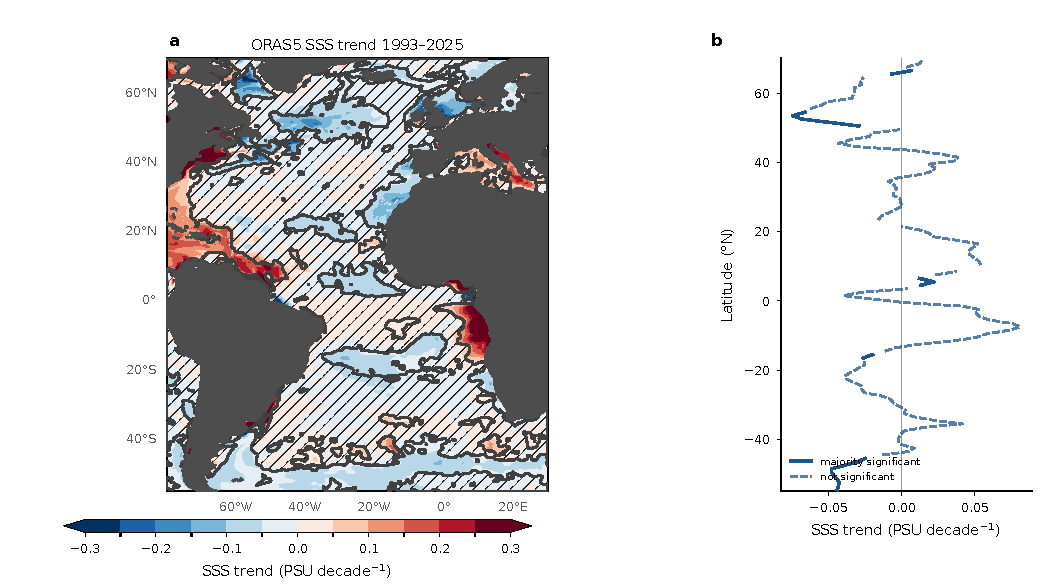
\includegraphics[width=0.94\textwidth]{../extended_data/ED1a_sss_trend_oras5.pdf}\\[0.4em]
  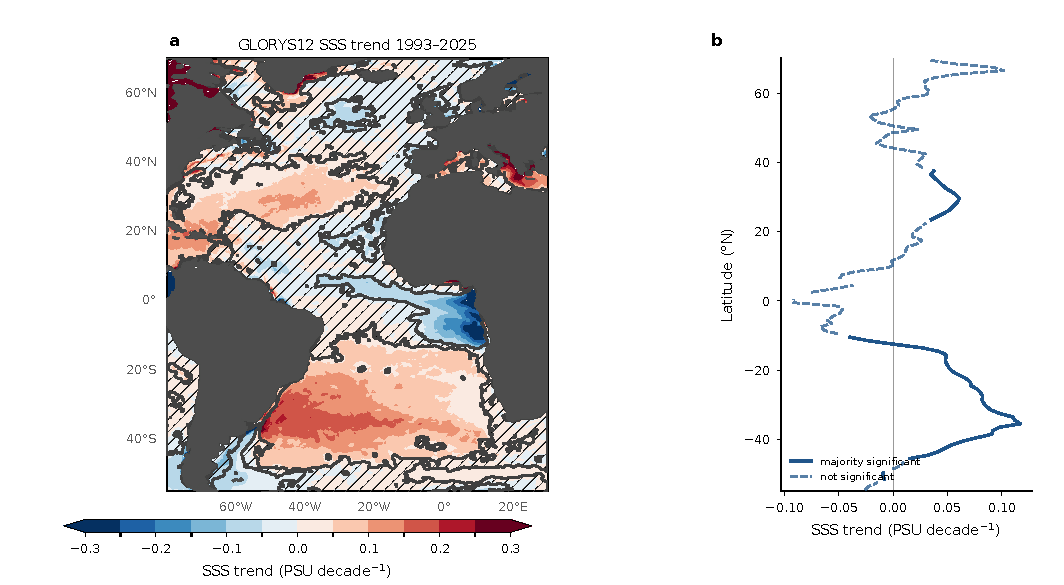
\includegraphics[width=0.94\textwidth]{../extended_data/ED1b_sss_trend_glorys12.pdf}
  \caption*{}
\end{figure}

\textbf{Extended Data Fig.~1 $\vert$ Surface salinity trends, 1993--2025.}
Per-pixel trends on deseasonalised monthly anomalies for ORAS5 and GLORYS12V1,
hatched where the Santer-adjusted $p$ exceeds 0.05. The effective-sample-size
correction reduces the significant ocean area from 76\% to 36\% in ORAS5 and
from 76\% to 51\% in GLORYS12V1. Atlantic band means disagree in sign between
the products in all three bands examined (60\degN{} to 80\degN{}, 40\degN{} to
60\degN{}, 10\degS{} to 35\degS{}), and only one of the six band-and-product
combinations is significant, GLORYS12V1 over 10\degS{} to 35\degS{}
($+0.061$~PSU per decade, $p=0.0002$). There is no significant subpolar North
Atlantic freshening in either product. \DIFdelbegin \DIFdel{A regression of band-mean salinity trend on band-mean salinity, the standard test for amplification of an existing
pattern, is not significant in either product ($R^2=0.06$, $p=0.24$ for
GLORYS12V1; $R^2=0.10$, $p=0.13$ for ORAS5), so these maps neither support nor
exclude a water-cycle origin for the changes\mbox{%DIFAUXCMD
\cite{Zika2018} }\hskip0pt%DIFAUXCMD
and }\DIFdelend \DIFaddbegin \DIFadd{Surface salinity trend patterns are in
any case ambiguous, since amplification of the water cycle and a uniform surface
heat flux both produce patterns resembling the one that would be attributed to
ocean transport\mbox{%DIFAUXCMD
\cite{Zika2018}}\hskip0pt%DIFAUXCMD
, which is why the argument in the main text rests
on the transport-weighted limb salinities at the section and these maps }\DIFaddend are not
used as evidence\DIFdelbegin \DIFdel{in the main text}\DIFdelend .

\begin{figure}[h]
  \centering
  \DIFdelbeginFL %DIFDELCMD < \includegraphics[width=0.80\textwidth]{../extended_data/ED2_streamfunction.pdf}
%DIFDELCMD <   %%%
\DIFdelendFL \DIFaddbeginFL 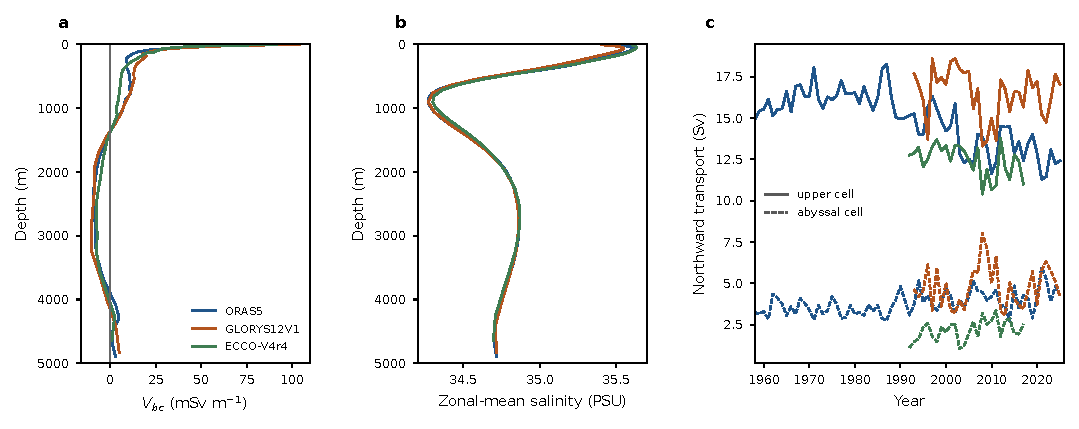
\includegraphics[width=0.98\textwidth]{../extended_data/ED2_section.pdf}
  \DIFaddendFL \caption*{}
\end{figure}

\textbf{Extended Data Fig.~2 $\vert$ \DIFdelbegin \DIFdel{Atlantic overturning streamfunction}\DIFdelend \DIFaddbegin \DIFadd{Section profiles and the structure of the
limbs}\DIFaddend .} \DIFaddbegin \textbf{\DIFadd{a}}\DIFadd{, }\DIFaddend Time-mean \DIFdelbegin \DIFdel{depth-space streamfunction for }\DIFdelend \DIFaddbegin \DIFadd{zonally integrated meridional velocity after
removal of the net section transport, over the matched 1993--2017 window. The
sign changes of this profile define the limbs. }\textbf{\DIFadd{b}}\DIFadd{, Time-mean zonally
averaged salinity over the same window. }\textbf{\DIFadd{c}}\DIFadd{, The northward-limb transport
split into its upper cell (solid) and its abyssal cell (dashed), on monthly
fields so that the two sum to $T$. The barotropic-corrected velocity changes sign
three to seven times in }\DIFaddend ORAS5 \DIFaddbegin \DIFadd{(modally four), three to four in GLORYS12V1 and
three to five in ECCO; the upper limb reaches to about 1325, 1245 }\DIFaddend and \DIFdelbegin \DIFdel{GLORYS12V1, showing the upper cell, the deep cell and the latitude of the upper-cell maximum. The
streamfunction is computed in depth coordinates by zonal integration of meridional velocity within the Atlantic basin mask, cumulated from the surface
downward, with the colour scale centred on zero. }%DIFDELCMD < 

%DIFDELCMD < \textbf{%%%
\DIFdel{Extended Data Table~1 $\vert$ CMIP6 model numbering for
Fig.~\ref{fig:cmip6}b.}%DIFDELCMD < \MBLOCKRIGHTBRACE %%%
\DIFdel{1 NESM3, 2 IPSL-CM6A-LR, 3 CNRM-CM6-1, 4 MIROC6, 5 MPI-ESM1-2-HR, 6 CanESM5, 7 UKESM1-0-LL, 8 CMCC-CM2-SR5, 9 GFDL-CM4, 10 ACCESS-CM2,
11 MPI-ESM1-2-LR, 12 HadGEM3-GC31-LL, 13 CESM2, 14 FIO-ESM-2-0, }\DIFdelend \DIFaddbegin \DIFadd{1318~m
respectively, and the abyssal limb begins at about 4044, 4405 and 4264~m. The abyssal cell carries 3.8, 4.8 and 2.2~Sv, that is 20\%,
23\% and }\DIFaddend 15\DIFdelbegin \DIFdel{GISS-E2-1-G, 16 FGOALS-g3}\DIFdelend \DIFaddbegin \DIFadd{\% of the northward limb, and is 0.21 to 0.49~PSU fresher than the
upper cell, which is why the redistribution between them has to be excluded
before the widening contrast can be read as a water-mass change. Its transport trend
is significant in ECCO ($+0.36$~Sv per decade, $p=0.041$) and in ORAS5
($+0.17$, $p=0.0004$), and not in GLORYS12V1}\DIFaddend .

\textbf{Extended Data Table~\DIFdelbegin \DIFdel{2 }\DIFdelend \DIFaddbegin \DIFadd{1 }\DIFaddend $\vert$ Reanalysis products.}

\begin{center}
\small
\begin{tabular}{lllll}
\toprule
 & ORAS5 & GLORYS12V1 & ECCO-V4r4 & SODA 3.15.2 \\
\midrule
Ocean model        & NEMO & NEMO & MITgcm & MOM5, SIS \\
Model resolution   & 0.25$^\circ$ & 1/12$^\circ$ & LLC90, $\sim$1$^\circ$ & 0.25$^\circ$ \\
Grid analysed      & native & native & 0.5$^\circ$ lat-lon & 0.5$^\circ$ Mercator \\
Vertical levels    & 75 & 50 & 50 & 50 \\
Assimilation       & NEMOVAR 3D-Var & reduced-order & \DIFdelbegin \DIFdel{4D-Var }\DIFdelend \DIFaddbegin \DIFadd{adjoint }\DIFaddend & optimal \\
                   & FGAT           & Kalman filter & \DIFdelbegin \DIFdel{adjoint }\DIFdelend \DIFaddbegin \DIFadd{(no increments) }\DIFaddend & interpolation \\
Atmospheric forcing & ERA-40, ERA-Interim, & ERA-Interim, & ERA-Interim & ERA5 \\
                    & ERA5 & ERA5 & (adjusted) & (COARE4) \\
\DIFdelbegin \DIFdel{$\Fovs$ record     }\DIFdelend \DIFaddbegin \DIFadd{Fields used        }& \DIFadd{816 monthly }& \DIFadd{396 monthly }& \DIFadd{312 monthly }& \DIFadd{43 annual }\\
\DIFadd{$T$, 1993--2017 (Sv) }& \DIFadd{17.9 }& \DIFadd{21.1 }& \DIFadd{14.6 }& \DIFadd{not recomputed }\\
\DIFadd{Record             }\DIFaddend & 1958--2025 & 1993--2025 & 1992--2017 & 1980--2022 \\
\DIFdelbegin \DIFdel{Records used       }\DIFdelend \DIFaddbegin \DIFadd{Ocean points       }\DIFaddend & \DIFdelbegin \DIFdel{816 monthly }\DIFdelend \DIFaddbegin \DIFadd{294 }\DIFaddend & \DIFdelbegin \DIFdel{396 monthly }\DIFdelend \DIFaddbegin \DIFadd{881 }\DIFaddend & \DIFdelbegin \DIFdel{26 annual }\DIFdelend \DIFaddbegin \DIFadd{146 }\DIFaddend & \DIFdelbegin \DIFdel{43 annual }\DIFdelend \DIFaddbegin \DIFadd{not recomputed }\\
\DIFadd{$T$ (Sv)           }& \DIFadd{18.7 }& \DIFadd{21.3 }& \DIFadd{14.6 }& \DIFadd{not recomputed }\\
\DIFadd{$\Delta S$ (PSU)   }& \DIFadd{$+0.068$ }& \DIFadd{$+0.136$ }& \DIFadd{$+0.307$ }& \DIFadd{not recomputed }\\
\DIFadd{Used quantitatively }& \DIFadd{yes }& \DIFadd{yes }& \DIFadd{yes }& \DIFadd{no }\DIFaddend \\
\bottomrule
\end{tabular}
\end{center}


\end{document}
